% $Id$

In this chapter, we present the results of a search for gravitational waves
from the inspiral of binary black hole MACHOs in data from the second LIGO
science run (called S2).  The goal of the search is the
detection of the gravitational waves. In the absence of a detection, however, we
place an upper limit on the rate of inspiralling BBHMACHOs. This
limit may be compared to the predicted rate of $5 \times 10^{-2} \times
2^{\pm 1}$ discussed in chapter \ref{ch:macho}.  

Analysis of the full S2 data set for gravitational waves from inspiralling
binary black hole MACHOs is complete and the result of this search will appear
in \cite{S2Macho:2004}. Since this result is currently embargoed pending LIGO
Scientific Collaboration internal review, we instead present the result of the
search on the playground data. No gravitational waves from BBHMACHO inspirals
were found in the playground, so in section \ref{s:s2upperlimit} we compute an
upper limit on the rate of binary black hole MACHO inspirals in the playground
data.  Although this result is statistically biased, as it is computed from
data used to tune the pipeline, it allows us to make a reasonable prediction
of the upper limit available using the full S2 data and assuming no BBHMACHO
signals are detected in the full data set.

In section \ref{s:s2run} we describe the data sample used in the analysis.
Section \ref{s:s2tuning} describes how the parameters of the search listed in
the previous chapter were tuned on the playground data. Section \ref{s:monte}
described the Monte Carlo simulations used to measure the efficiency of the
pipeline. In section \ref{s:s2background} we describe the background observed
in the S2 data.


\section{The Second LIGO Science Run}
\label{s:s2run}

All three LIGO detectors operated during the second science run, referred to
as S2, which lasted for 59 days (1415 hours) from February 14 to April 14,
2003.  Although the detectors were manned by operators and scientific monitors
around the clock, the amount of data flagged for scientific analysis was
limited by environmental factors (especially high ground motion at LLO and
strong winds at LHO), occasional equipment failures, and periodic special
investigations.  The total amount of science data obtained was 536 hours for
L1, 1044 hours for H1, and 822 hours for H2.

The analysis described in this thesis uses data collected while the LLO
detector was operating at the same time as one or both of the LHO detectors in
order to make use of the triggered search pipeline.  Science mode data during
which both H1 and H2 were operating but L1 was not, amounting to 383 hours,
was not used in this analysis because of concerns about possible
environmentally-induced correlations between the data streams of these two
co-located detectors. This data set, as well as data collected while only one
of the LIGO detectors was in science mode, will be combined with data from the
third LIGO science run in a future analysis. Figure~\ref{f:S2times} shows a
breakdown by interferometer of the data recorded during S2. The data used in
this search is indicated by the shaded region.

\section{Tuning the Analysis Pipeline}
\label{s:s2tuning}

The entire analysis pipeline was explored first using the playground data set
in order to tune the the various thresholds and other parameters. The goal of
tuning the pipeline is to maximize the efficiency of the pipeline to detection
of gravitational waves from binary inspirals without producing an excessive
rate of spurious candidate events. In the absence of a detection, a pipeline
with a high efficiency and low false alarm rate allows us to set the best
upper limit. It should be noted, however, that our primary motivation is to
enable reliable detection of gravitational waves. The efficiency is measured
by Monte Carlo simulations in which signals from the hypothetical population
are added to the data and then sought. This approach accounts for any
systematic error associated with the methods used in our pipeline.  Note that
another factor in the tuning of the pipeline are the available computational
resources. We would like to be able to complete the search in less time than
the length of the data being analyzed, so that real-time searches are possible
when the interferometers are taking continuous data. For this reason, certain
tuning decisions are based on the computational efficiency of the pipeline;
these decisions will be clearly identified below.

Prior to commencing the binary black hole MACHO search, a search for
inspiralling binary neutron stars (BNS) was conducted on the S2 data using the
pipeline described in chapter~\ref{ch:pipeline}\cite{LIGOS2iul}. The mechanics
of the BNS search are very similar to those described here, except that the
template bank covers binaries with $1.0\,M_\odot < m_1, m_2 < 3.0\,M_\odot$,
where $m_1$ and $m_2$ are the masses of each object in the binary. Since the
BNS and binary black hole MACHO searches are very similar, and share the same
playground data, we may use the parameters of the BNS search (which were tuned
on the playground data) as a starting point for tuning the binary black hole
MACHO search. 

There are two sets of parameters that we are able to tune in the pipeline: (i)
the single interferometer parameters which are used in the matched filter and
$\chi^2$ veto to generate inspiral triggers in each interferometer, and (ii)
the coincidence parameters used to determine if triggers from two
interferometers are coincident. The single interferometer parameters include
the signal-to-noise threshold $\rho^\ast$, the number of frequency sub-bands in
the $\chi^2$ statistic $p$, the $\chi^2$ cut threshold $\Xi^\ast$,  and the
coefficient on the signal-to-noise dependence of the $\chi^2$ cut, i.e.
$\delta^2$ in equation (\ref{eq:chisqthresholdtest}). These are tuned on a
per-interferometer basis, although some of the values chosen are common to two
or even three detectors.  The coincidence parameters are the time coincidence
window $\delta t$ for triggers, the mass parameter coincidence window $\delta
m$ and the effective distance cut parameters $\epsilon$ and $\kappa$ in
equation.~(\ref{eq:eff_dist_test}).  Due to the nature of the triggered search
pipeline, parameter tuning was carried out in two stages. We first tuned the
single interferometer parameters for the primary detector (L1).  We then used
the triggered template banks (generated from the L1 triggers) to explore the
single interferometer parameters for the less sensitive Hanford detectors.
Finally the parameters of the coincidence test were tuned.

\subsection{Template Bank Generation}
\label{ss:tunebank}

Recall that the number of templates needed to cover a given region of
parameter space at a specified minimal match fluctuates as the shape of the
noise power spectrum changes. The greater the sensitivity at low frequencies,
relative to higher frequencies, the larger the template bank (see section
\ref{ss:templatebank}). The computational resources available for the MACHO
search are limited and the computational cost is proportional number of
templates in the bank. We therefore tuned the template bank parameters to
allow the search to be completed within the available resources.

Due to the algorithm used to construct the template bank\cite{Owen:1998dk}, the
smallest mass template in the bank will be the equal mass binary
$(m_\mathrm{min},m_\mathrm{min})$, where $m_\mathrm{min}$ is the (user
specified) minimum binary component mass. Figure~\ref{f:bank_size} shows the
size of the template bank necessary to cover each playground analysis chunk at
a minimal match of $0.97\%$ for several values of $m_\mathrm{min}$.  The
maximum binary component mass in each case is $1\,M_\odot$, so the largest
mass binary in the bank parameter space is $(1,1)\,M_\odot$. For fixed
$m_\mathrm{min}$ the number of templates remains reasonably constant over the
course of the S2 run, but there is a large variation in the number of templates
required as a function of lower mass. The scaling of template number
as a function of lower mass is consistent with that described in
\cite{Owen:1998dk}.

As described in chapter \ref{ch:macho}, the MACHO mass range measured by
microlensing is $0.15\,M_\odot$ to $0.9\,M_\odot$ at $95\%$ confidence. It
would therefore be desirable for the binary black hole MACHO inspiral search
to cover a region of mass parameter space slightly larger than this, say
$0.1\,M_\odot$ to $1.0\,M_\odot$.  It can be seen, however, that almost an
order of magnitude more templates are needed to decrease the lower boundary of
the mass parameter space from $0.2\,M_\odot$ to $0.1\,M_\odot$.  Therefore,
given the computational resources available for the BBHMACHO search, the
lowest mass template in the bank was set to $0.2\,M_\odot$. Note that for the
final search, the match of the template bank was also lowered to $0.95\%$ to
further decrease the number of templates to an average of $14\,179$ per
analysis chunk over the S2 run.  The latter choice is be justified by the
sensitivity to galactic binary black hole MACHOs in S2, as will be seen below.
The size of the inspiral template bank used is shown in
figure~\ref{f:inspiral_summary}.
 
\subsection{Interferometer Sensitivity and Signal-to-noise Thresholds}
\label{ss:snrthreshold}

The noise power spectrum also determines the sensitivity of the interferometer
to binary inspirals. We can quantify the sensitivity in terms of the distance
to which we can see an optimally oriented binary inspiral at a given
signal-to-noise ratio. This is the maximum distance at which the
interferometer can detect a binary (at this signal-to-noise ratio), since the
gravitational wave strain in the interferometer is a maximum when the binary
is optimally oriented.  The maximum inspiral ranges for an optimally oriented
binary at signal-to-noise ratio $\rho^\ast = 8$ are shown in
figure~\ref{f:inspiral_summary}.  The distance to which we can detect an
optimally oriented binary is also a function of the mass of the binary,
scaling as $\mu^{1/2}M^{1/3}$; figure~\ref{f:inspiral_summary} shows the
ranges for a $(0.5,0.5)\,M_\odot$ and a $(0.1,0.1)\,M_\odot$ binary.

Notice that there are no times when either of the LHO interferometers are more
sensitive than the LLO interferometer and so demanding triggers are always
present in the most sensitive interferometer means that they are required to
be found in L1. In fact the LLO interferometer has a significantly larger
range than either of the LHO interferometers, at times being sensitive to
BBHMACHO inspirals in Andromeda at around $0.7$~Mpc.  Since we require
coincidence between L1 and one of the LHO interferometers to make a detection,
however, we are restricted to a search for BBHMACHOs in the Galactic halo.  

Based on the sensitivity plots shown in figure~\ref{f:inspiral_summary}, we
set the signal-to-noise threshold to $7$ in all three interferometers; we
justify this as follows. All three interferometers are sensitive to optimally
oriented inspirals with $\rho^\ast \ge 8$ at distances greater than the size
of the Galactic halo. A binary black hole MACHO in the Galaxy may have an
unfavorable orientation, however, causing it to appear at a large effective
distance.  For this reason, we want to set the signal-to-noise ratio threshold
as low as possible without producing an excessive false alarm rate. Lowering
the signal-to-noise threshold has a computational impact on our search:
when the signal-to-noise ratio for a template crosses threshold, we
perform the $\chi^2$ veto which requires $p$ additional complex inverse FFTs,
where $p$ is the number of frequency bins used in the veto. If we set the
signal-to-noise threshold too low, we may exceed the available computational
resources due to the extra operations required to perform the $\chi^2$ veto.
In fact this is what happens with the S2 binary black hole MACHO search since
the template banks are so large. Whereas in the S2 BNS search we were able to
lower the signal-to-noise threshold to $6$, the BBHMACHO search is limited to
a signal-to-noise threshold to $7$.

\subsection{Tuning the $\chi^2$ Veto Parameters}
\label{ss:chisqtuning}

%Recall that the $\chi^2$ veto constructs the quantity
%\begin{equation}
%\Xi = \frac{\chi^2}{p + \delta^2\rho^2}
%\end{equation}
%and accepts triggers that pass the test $\Xi < \Xi^\ast$, where $\Xi^\ast$ is
%the threshold, as described in section~\ref{s:chisqcts}.
%The initial parameters used for the $\chi^2$ veto, based on tuning of the BNS
%search, were $p = 15$ and $\delta^2 = 0.04$ with the threshold set to
%$\Xi^\ast_\mathrm{L1} = 5.0$ in the L1 interferometer and
%$\Xi^\ast_\mathrm{H1} = \Xi^\ast_\mathrm{H2} = 12.5$ in the LHO
%interferometers. 

Recall from section~\ref{ss:mismatchedchisq} that the $\chi^2$ veto thresholds
on
\begin{equation}
\chi^2 < \chi^2_\ast (p+\rho^2 \delta^2),
\label{eq:chisqthreshold2}
\end{equation}
where $\rho$ is the signal-to-noise ratio of the signal and $\delta^2$ is a
parameter chosen to be reflect the largest expected mismatch that a true
signal will have with the templates in the bank. The initial parameters used
for the $\chi^2$ veto, based on tuning of the BNS search, were $p = 15$ and
$\delta^2 = 0.04$ with the threshold set to $\chi^2_\ast(\mathrm{L1}) = 5.0$ in
the L1 interferometer and $\chi^2_\ast(\mathrm{H1}) = \chi^2_\ast(\mathrm{H2}) =
12.5$ in the LHO interferometers.

Figure \ref{f:h1_chiqsq_tuning} illustrates tuning of the $\chi^2$ veto on the
H1 playground triggers. If the interferometer noise is Gaussian, then the
square of the signal-to-noise ratio should be $\chi^2$ distributed with two
degrees of freedom. This means that the histogram of the signal-to-noise ratio
of the triggers should be a monotonically decreasing function of $\rho$. We
can see from figure~\ref{f:h1_chiqsq_tuning}, however, that there is an excess
in the number of triggers with $\rho \approx 8.5$; this suggests some
non-Gaussian behavior in the data that we would like to remove. It can be seen
that decreasing the threshold $\chi^2_\ast$ to $5$ removes this hump in the
distribution and decreases the signal-to-noise ratio of the loudest event from
$\rho = 13.8$ to $\rho = 10.7$. This suggests that lowering the $\chi^2$
threshold is desirable.  Figure~\ref{f:h1_missed_tuning}, which shows the
results of a small Monte Carlo simulation, demonstrates the danger of making
such decisions without reference to the detection efficiency, however. For
each simulated signal added to the data, the figure shows whether or not it was
detected in the H1 data using the initial choice of $\chi^2$ veto parameters
($\delta^2 = 0.04$, $\chi^2_\ast(\mathrm{H1}) = 12.5$). Several injections are
missed at effective distances well within the range of the H1 interferometer.
Follow up investigations of these missed triggers show that, although they
have very large values of signal-to-noise $\rho \sim 10^2 - 10^3$, they are
missed because they fail the $\chi^2$ veto. This is caused by the mismatch
between the signal and the template.  The results of this study imply that we
should loosen the $\chi^2$ veto, in contradiction to the results suggested by
figure~\ref{f:h1_chiqsq_tuning}.  Notice, however, that the excess of H1
triggers occurs at low values of $\rho$ and the missed injections are at
higher values of $\rho$. Figure~\ref{f:h1_inj_xi_tuning} shows the values of
$\chi^2/(p+\rho^2\delta^2)$ and $\rho$ for the detected L1 injections and the
detected H1 injections before coincidence is applied. These triggers are taken
from the same Monte Carlo simulation as the triggers shown in
figure~\ref{f:h1_missed_tuning}. The values of $\chi^2/(p+\rho^2\delta^2)$
observed for the detected H1 injections are significantly higher than those
for the L1 injections. This suggests that we should increase the parameter
$\delta^2$, which has the effect of decreasing the value of
$\chi^2/(p+\rho^2\delta^2)$ for triggers with high signal-to-noise ratios. If
we increase $\delta^2$ we may be able to decrease the value of
$\chi^2/(p+\rho^2\delta^2)$ to remove the excess of triggers in H1, without
adversely affecting the pipeline detection efficiency. After several
iterations, the values $\delta^2 = 0.4$, $\chi^2_\ast(\mathrm{L1}) = 3.1$,
$\chi^2_\ast(\mathrm{H1}) = 5.0$ and $\chi^2_\ast(\mathrm{H2}) = 10.0$ were
chosen.  Figure~\ref{f:h1_inj_xi_final} shows the values of $\Xi$ and $\rho$
for the detected L1 injections and the detected H1 injections with these new
parameters. Notice that the values of $\chi^2/(p+\rho^2\delta^2)$ for the loud
signal-to-noise triggers are considerably lower than before. It appears from
the results in figure~\ref{f:h1_inj_xi_final} that it would be possible to
reduce $\chi^2_\ast(\mathrm{H1})$ further to $2.51$, without loss of
efficiency. No coincident triggers survived the pipeline in the playground
data with a threshold of $\chi^2_\ast(\mathrm{H1}) = 5.0$, however, so it was
decided not to reduce this threshold further.

\subsection{Coincidence Parameter Tuning}
\label{ss:coinc_tuning}

After the single interferometer parameters had been selected, the coincidence
parameters were tuned using the triggers from the single interferometers.  As
described in section~\ref{ch:hardware}, the coalescence time of an inspiral
signal can be measured to within $\le1$~ms. The light travel time between
observatories is $10$~ms, so $\delta t$ was chosen to be $1$~ms for LHO-LHO
coincidence and $11$~ms for LHO-LLO coincidence. The mass coincidence
parameter was initially chosen to be $\delta m = 0.03$, however testing with
the binary neutron star search showed that this could be set to $\delta m =
0.0$ ({\it i.e.}\ requiring the triggers in each interferometer to be found
with the exact same template) without loss of efficiency.

Having tuned the time and mass parameters, we tune the effective
distance parameters $\kappa$ and $\epsilon$. Initial estimates of $\epsilon =
2$ and $\kappa = 0.2$ were used for testing, however it was discovered that
many injections were missed using these thresholds to test for LLO-LHO
coincidence. This is due to the fact that the detectors are slightly
misaligned, so the ratio of effective distance of a trigger between the two
observatories can be large for a significant fraction of the population, as
shown in Fig.~\ref{f:gmst_dist_ratio}. As a result, we disabled the
effective distance cut for triggers generated at different observatories.
A study of simulated signals injected into H1 and H2 interferometers, both
located at the LIGO Hanford Observatory, suggested using values
of $\epsilon_{HH} = 2$ and $\kappa_{HH} = 0.5$. Note
that, as described above, we demand that an L1/H1 trigger pass the H1/H2
coincidence test if the effective distance of the trigger in H1 is within the
maximum range of the H2 detector at threshold.

\section{Results of Injection Monte Carlo Simulations}
\label{s:monte}

The final parameter values chosen are shown in table~\ref{t:ifo_params}. Once
fixed, an injection Monte Carlo was performed to measure the efficiency of the
search pipeline. For each playground interval in the S2 data, an inspiral
waveform was generated using the population model described in
section~\ref{s:bbhmachopopulation}. These signals has masses between
$0.1\,M_\odot$ and $1.0\,M_\odot$. Each inspiral signal was injected into the
data at a random time during a unique playground interval and the data
analyzed through the full pipeline with the final set of parameters. Four
separate simulation runs were performed giving a total of 849 injections in
the analyzed playground data.  Figure~\ref{f:m1m2_found_missed} shows the
results of this simulation in the $(m_1,m_2)$ plane. The figure shows which of
the simulated signals were detected and which were missed by the full pipeline
in the double and triple coincident playground data. Also shown in the figure
is the effective distance at which these signals were injected in the LHO
interferometers, since it is generally the less sensitive detector that limits
the detection efficiency.  Although the template bank only coves the region
above and to the right of the red lines at $0.2\,M_\odot$, the upper plot
shows that some signals are detected with component masses between $\sim
0.15$--$0.20\,M_\odot$. This is a direct result of increasing $\delta^2$ in
the $\chi^2$ veto, equation (\ref{eq:chisqthreshold2}), allowing loud, but
slightly mismatched signals to be detected. The lower plot in
figure~\ref{f:m1m2_found_missed} shows the injections that are missed by
the pipeline. Injections missed from triple, L1-H1 double and L1-H2 double
coincident data are shown with a star, an upward triangle and a downward
triangle respectively. These missed signals are color coded with the injected
effective distance in the LHO detectors. Injections are
only missed when their effective distance is comparable or greater than the
ranges for the LHO detectors shown in figure~\ref{f:inspiral_summary}; there
are no anomalous missed injections.  Figure~\ref{f:mchirp_eff} shows the
efficiency of the search as a function of chirp mass. As expected, given the
strength of the BBHMACHO signals and the sensitivity of the detectors, the
efficiency is $\varepsilon \sim 1$ for $\mathcal{M} >0.35$ with the small loss
of efficiency coming from systems with an unfavorable orientation. The
efficiency drops for $\mathcal{M}$ below $0.35$ due to the combined effect
of the signals becoming weaker as the chirp mass decreases and falling outside
the region of good template bank coverage.  Notice that there appears to be an
anomalous value of $\varepsilon$ at $\mathcal{M} \approx 0.2$; this appears to
be associated with a dearth of injections in this mass range.  Large scale
Monte Carlos, with many more injections, are currently being performed to
explore this region of parameters space and investigate this anomaly in the
full S2 data set.

A comparison of the inspiral parameters recovered by the pipeline and the
known injection parameters from signals injected in the Monte Carlo simulation
are shown for L1, H1 and H2 in figures \ref{f:l1_param_error},
\ref{f:h1_param_error} and \ref{f:h2_param_error} respectively. It can be seen
that the effective distance recorded by the search code is unbiased in all
cases, and can typically be recovered to an accuracy of $\sim 10\%$. This is
comparable to the $10\%$ distance uncertainty to nearby galaxies.  Using the
measured coalescence phase, effective distance and difference in time of
arrive at the two detectors, it is possible to gain information about the
location of the signals, however a comprehensive study of this has not been
performed for the S2 data. For all interferometers, the chirp mass is
recovered extremely well with an accuracy of $0.1\%$. This consistent with the
results quoted in \cite{Cutler:1994} and is encouraging for the parameter
measurement in the case of a detection. Although there appears to be a bias in
the measure end time of the signal, this is due to the fact that the current
implementation of the filtering code measures the end time of the template,
not the coalescence time of the binary. The injected signals are generated
with a time domain waveform generator\cite{LAL} and recovered with the
stationary phase waveforms described in chapter \ref{ch:findchirp}. There is a
slight difference in the frequency at which these waveforms terminate: the
time domain waveforms are terminated when the post-Newtonian phase evolution
of equation (\ref{eq:biwwphase}) can no longer be evolved and the stationary
phase waveforms are terminated when they reach the gravitational wave
frequency of a test particle in the innermost stable circular orbit of
Schwarzschild spacetime. As a result of this there is a small mass dependent
offset between the end times of the waveform as recorded by the injection code
and the filtering code. This will not affect the time coincidence test,
however, as we demand that the templates have the same mass parameters
in all the detectors. As a result this time offset will be identical between
detectors and we can apply coincidence. Changes to the filtering code are
planed to remove this offset in time measurement.

\section{Background Estimation}
\label{s:s2background}

We estimate the background rate for this search by introducing an artificial
time offset, or {lag}, $\Delta t$ in the triggers coming from the Livingston
detector relative to the Hanford detector.  The time-lag triggers are then fed
into subsequent steps of the pipeline.  The triggers that emerge from the end
of the pipeline are considered a single trial representative of an output from
a search if no signals are present in the data.   By choosing a lag of more
than 20~ms, we ensure that a true gravitational wave will not be coincident in
the time-shifted data streams.  We do not time-shift the two Hanford detectors
relative to one another since there may be real correlations due to
environmental disturbances.  If the times of background triggers are not
correlated at the sites, then the background rate can be measured. A total of
20 time-lags were analyzed to estimate the background. Note that the time lags
use all the data and are not restricted to playground. The resulting
distribution of time-lag triggers in the
$(\rho_{\mathrm{H}},\rho_{\mathrm{L}})$ plane is shown in figure~\ref{f:bkg};
the distribution of background triggers and injected signals are compared in
figure~\ref{f:bkg_inj}. It can be seen that the signal-to-noise ratios of
background triggers are higher in the LHO interferometers than in the L1
interferometer, whereas the signal-to-noise ratios of injections are louder in the
L1 interferometer. This distribution suggested the form of a ``coherent''
signal-to-noise ratio $\hat{\rho}$ which gives a factor of 2 more significance
to the signal-to-noise ratio in L1 compared to the signal-to-noise ratio in
L1. Based on the studies of the background and injections, we chose a
combined signal-to-noise statistic
\begin{equation}
\hat{\rho}^2 = \rho^2_{\mathrm{L1}} +  \frac{\rho_{\mathrm{H}}^2 }{ 4 }.
\label{eq:combinedsnr}
\end{equation}

\section{Upper Limit on BBHMACHO Inspiral in the S2 Playground Data}
\label{s:s2upperlimit}

After the data quality cuts, discarding science segments with durations
shorter than 2048 sec, and application of the instrumental veto in L1, a
total of {35.2} hours of playground data remained; {22.0} hours of
triple-detector data,  {10.2} hours of L1-H1 and {3.97} hours of L1-H2. The
analysis of the playground data produced no double or triple coincident
inspiral candidates.

To determine an upper limit on the event rate we use the \emph{loudest event
statistic}\cite{loudestGWDAW03} which uses the detection efficiency at the
signal-to-noise ratio of the loudest trigger surviving the pipeline to
determine an upper limit on the rate. If no triggers survive the pipeline, we
use the signal-to-noise threshold as the loudest event.  Suppose the
population of sources produces Poisson-distributed events with a rate
$\mathcal{R}$ per year per Milky Way Equivalent Galaxy (MWEG) and
$N_G(\rho^\ast)$ is the number of MWEGs to which the search is sensitive at
$\rho \geq \rho^\ast$.   Then the probability of observing an inspiral signal
with $\rho > \rho^\ast$, given some rate $\mathcal{R}$ and some observation
time $T$, is
\begin{equation}
P(\rho>\rho^\ast;{\mathcal{R}}) = 1 - e^{-{\mathcal{R}}T N_G(\rho^\ast)}.
\label{eq:foreground-poisson}
\end{equation}
A trigger can arise from either an inspiral signal in the data or from
background.   If $P_b$ denotes the probability that all background triggers
have signal-to-noise ratio less than $\rho^\ast$,  then the probability of observing either an
inspiral signal or a background trigger with $\rho > \rho^\ast$ is given by
\begin{equation}
P(\rho>\rho^\ast;{\mathcal{R}},b) = 1 - P_b e^{-{\mathcal{R}}TN_G(\rho^\ast)}.
\label{eq:joint-dist}
\end{equation}
Given the probability $P_b$, the total observation time $T$, and the number of
Milky Way equivalent galaxies $N_{{G}}$ to which the search is sensitive, we
find that the rate of binary black hole MACHO inspirals per MWEG is
\begin{equation}
  R_{90\%} = \frac{2.303+\ln P_b}{T N_{G}(\rho^\ast)}
\end{equation}
with 90\% confidence. This is a frequentist upper limit on the rate.
For ${\mathcal{R}}>{\mathcal{R}}_{90\%}$, there is more than $90\%$
probability that at least one event would be observed with SNR greater
than $\rho_{\text{max}}$. 

Since no coincident events were observed in the playground data, we determine
the rate by measuring the efficiency of the pipeline at the (combined)
signal-to-noise threshold
\begin{equation}
\hat{\rho}^2_\mathrm{max} =  7^2 + \frac{7^2}{4} = 61.25.
\label{eq:threshold}
\end{equation}
This is a conservative limit on the rate. If we lowered the
signal-to-noise thresholds until we observed the loudest trigger, then this
trigger will have a signal-to-noise ratio less than the value given in equation
(\ref{eq:threshold}); the measured efficiency will be greater than or equal to
that used here so the rate will be less than or equal to which we
quoted here. Furthermore, since we only have a small number of time lags, we
neglect the background term $P_b$. Dropping this term will give a conservative
value for upper limit\cite{loudestGWDAW03}.

If we restrict the mass parameters of the injected signals to those with a
component in the range $0.15$ to $1.0\,M_\odot$, the mass range suggested by
microlensing observations, we find that efficiency of the search pipeline at
$\hat{\rho}^\ast = \sqrt{61.25}$ is 
\begin{equation}
\varepsilon\left( \hat{\rho}^\ast = \sqrt{61.25} \right) = \frac{ 692 } { 756
} = 0.915.
\end{equation}
The observation time for the playground data is $T = 35.2\,\mathrm{hours} = 4
\times 10^{-3}\,\mathrm{yr}$ and so the upper limit on the rate of binary
black hole MACHO inspirals in the playground data is
\begin{equation}
\mathcal{R}_{90\%} = \frac{2.303}{0.915 \times 4 \times 10^{-3}} = 
627\,\mathrm{yr}^{-1}\,\mathrm{MWEG}^{-1}.
\end{equation}

The amount of non-playground data in the full S2 data, again discarding
science segments with durations shorter than 2048 sec,  and application of the
instrumental veto in L1, there is a total of 345 hours of non-playground data;
225 hours of triple-detector data, 90 hours of L1-H1 and 30 hours of L1-H2.
Assuming that the signal-to-noise ratio of the loudest event in the full data
is comparable to $\hat{\rho}^2 = 61.25$, which is suggested by the background
triggers, we may estimate the achievable upper limit as
\begin{equation}
R_{90\%} = \frac{2.303}{0.915 \times 3.9 \times 10^{-2}} = 
64\,\mathrm{yr}^{-1}\,\mathrm{MWEG}^{-1}.
\end{equation}
This upper limit is three orders of magnitude larger than the upper bound on
the rate of $R = 0.05\times2^{\pm 1}\,\mathrm{yr}^{-1}\,\mathrm{MWEG}^{-1}$,
so we are not yet able to constrain the fraction of the Galactic halo in
BBHMACHOs. The sensitivity of the interferometers during the S2 search is
roughly an order of magnitude from design sensitivity, however. For a
$(0.5,0.5)\,M_\odot$ binary, at design sensitivity the interferometers will be
sensitive to $\sim 50$~MWEG, so in one year of data taking, assuming no
detections have been made, an upper limit on rate of BBHMACHO inspirals of $R
= 3\times10^{-2}\,\mathrm{yr}^{-1}\,\mathrm{MWEG}^{-1}$ are possible (assuming
$P_b = 0.5$) which will significantly impact the theoretical rate estimates.
Additionally, since the range of the search scales as a function of the mass,
the possibility for detecting more massive BBHMACHO binaries increases as more
galaxies become accessible and the rate can be further constrained.

%%%%%%%%%%%%%%%%%%%%%%%%%%%%%%%%%%%%%%%%%%%%%%%%%%%%%%%%%%%%%%%%%%%%%%%%%%%%%%%

\newpage

\begin{figure}[p]
\begin{center}
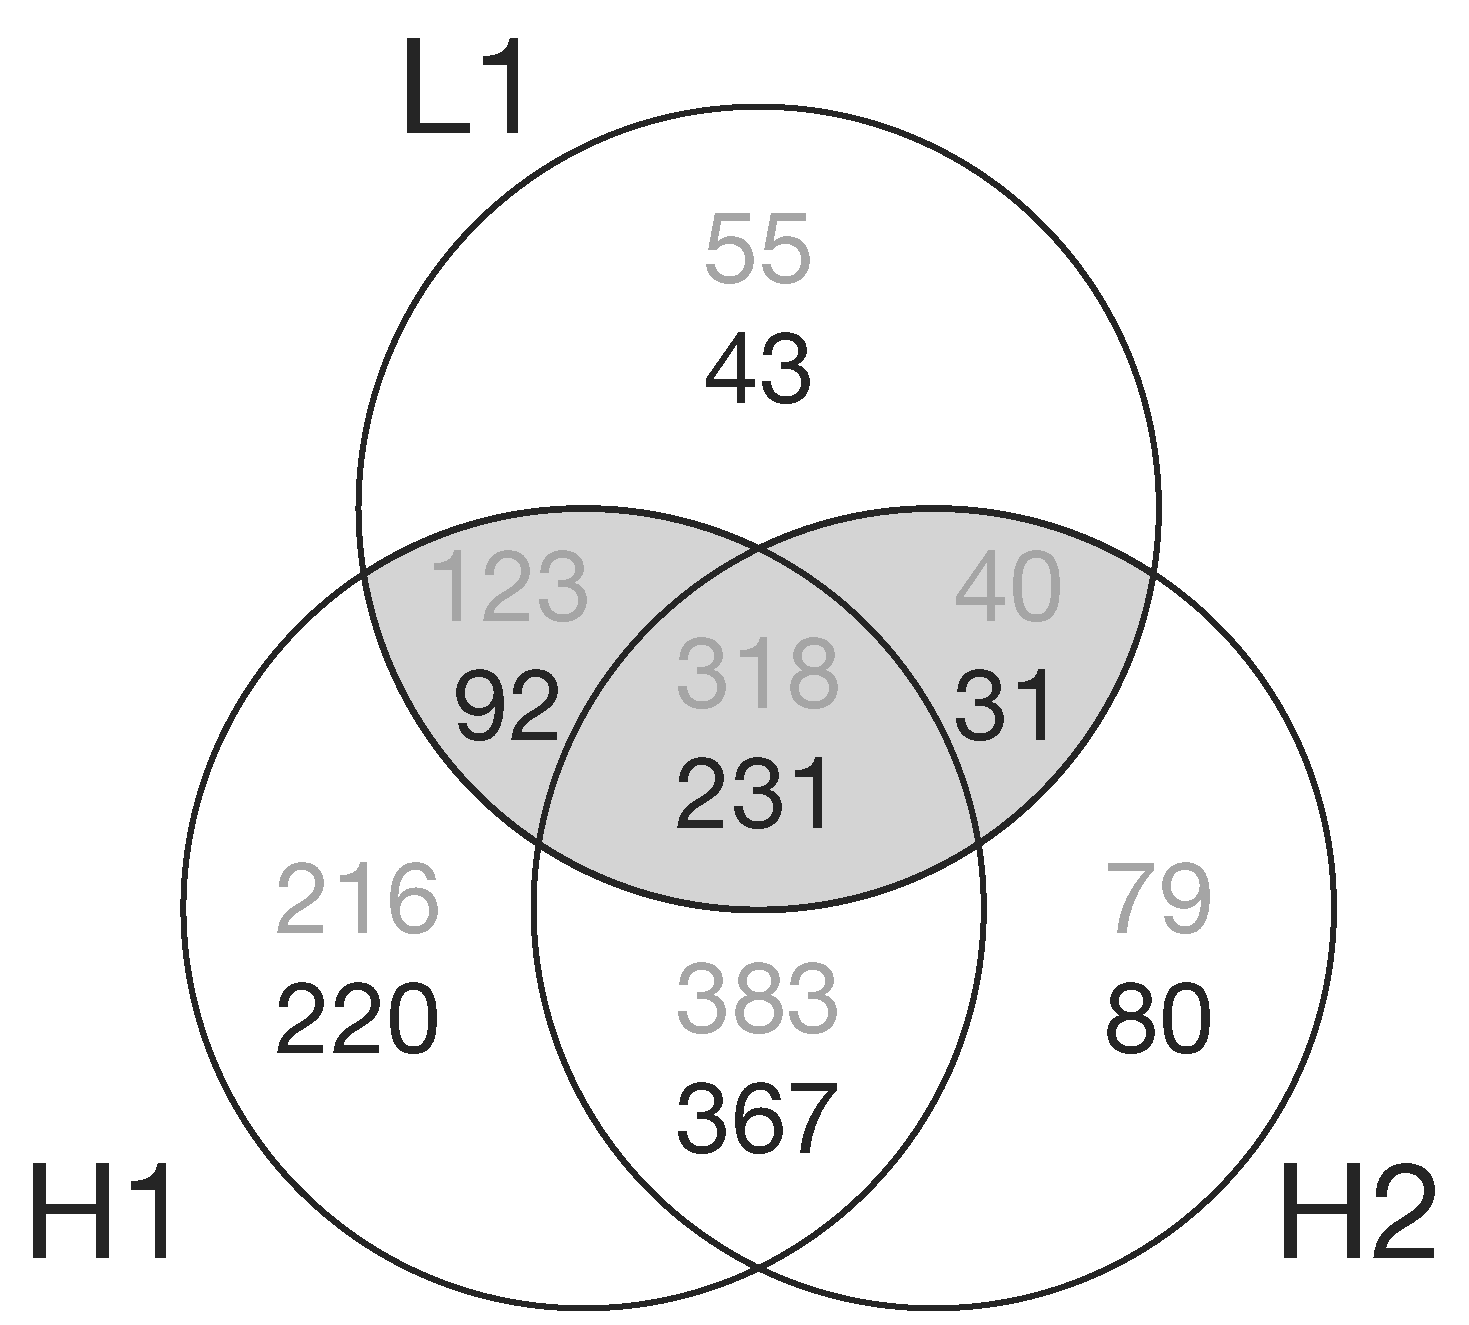
\includegraphics[width=0.75\linewidth]{figures/result/s2_times}
\end{center}
\caption[Amounts of Single and Coincident Interferometer Data in S2]{%
\label{f:S2times}%
The Venn diagram shows the number of hours that each detector combination was
operational during the S2 run.  The upper number gives the amount of time the
specific instruments were operational.  The lower number gives the total
non-playground time which was searched for inspiral triggers.  The shaded
region corresponds to the data used in the S2 MACHO search.}
\end{figure}

\begin{figure}[p]
\begin{center}
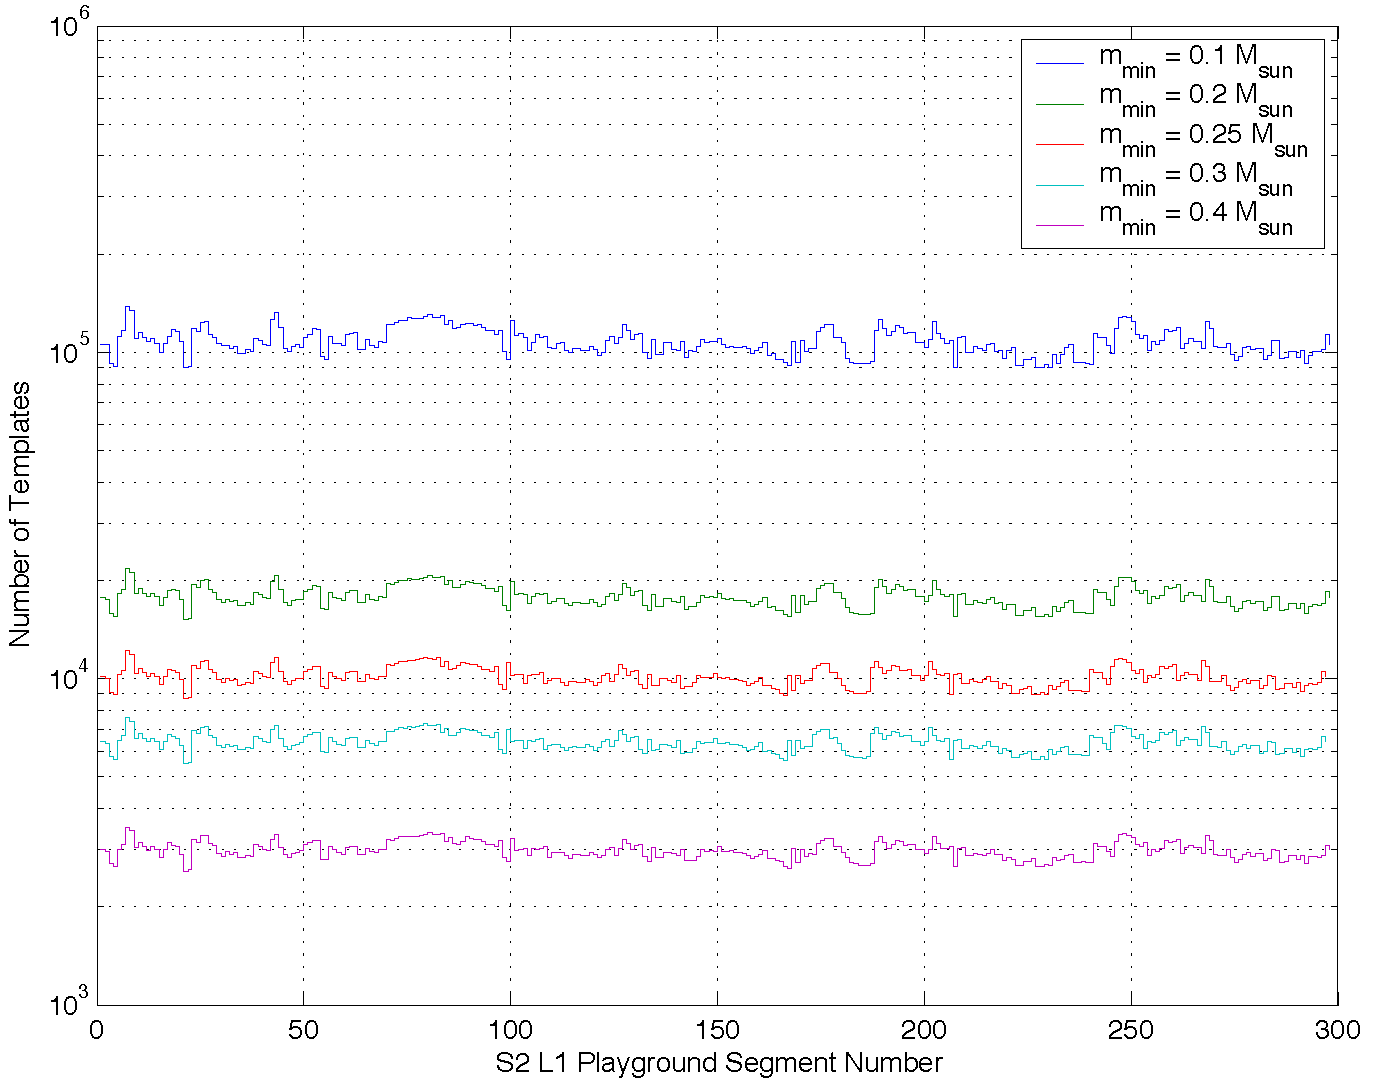
\includegraphics[width=\linewidth]{figures/result/bank_size}
\end{center}
\caption[MACHO Template Bank Size for Various Lower Masses]{%
\label{f:bank_size}%
The plot shows the size of the template bank, generated with a minimal match
of $97\%$, for various values of $m_\mathrm{min}$. As described in section
\ref{ss:templatebank} the size of the template bank is proportional to
$m_\mathrm{min}^{-8/3}$, where $m_\mathrm{min}$ is the mass parameter of the
smallest equal mass binary in the template bank. Using these data, it was
decided that the lowest mass accessible was $m_\mathrm{min} = 0.2\,M_\odot$,
given the available computational resources.}
\end{figure}

\begin{figure}[p]
\begin{center}
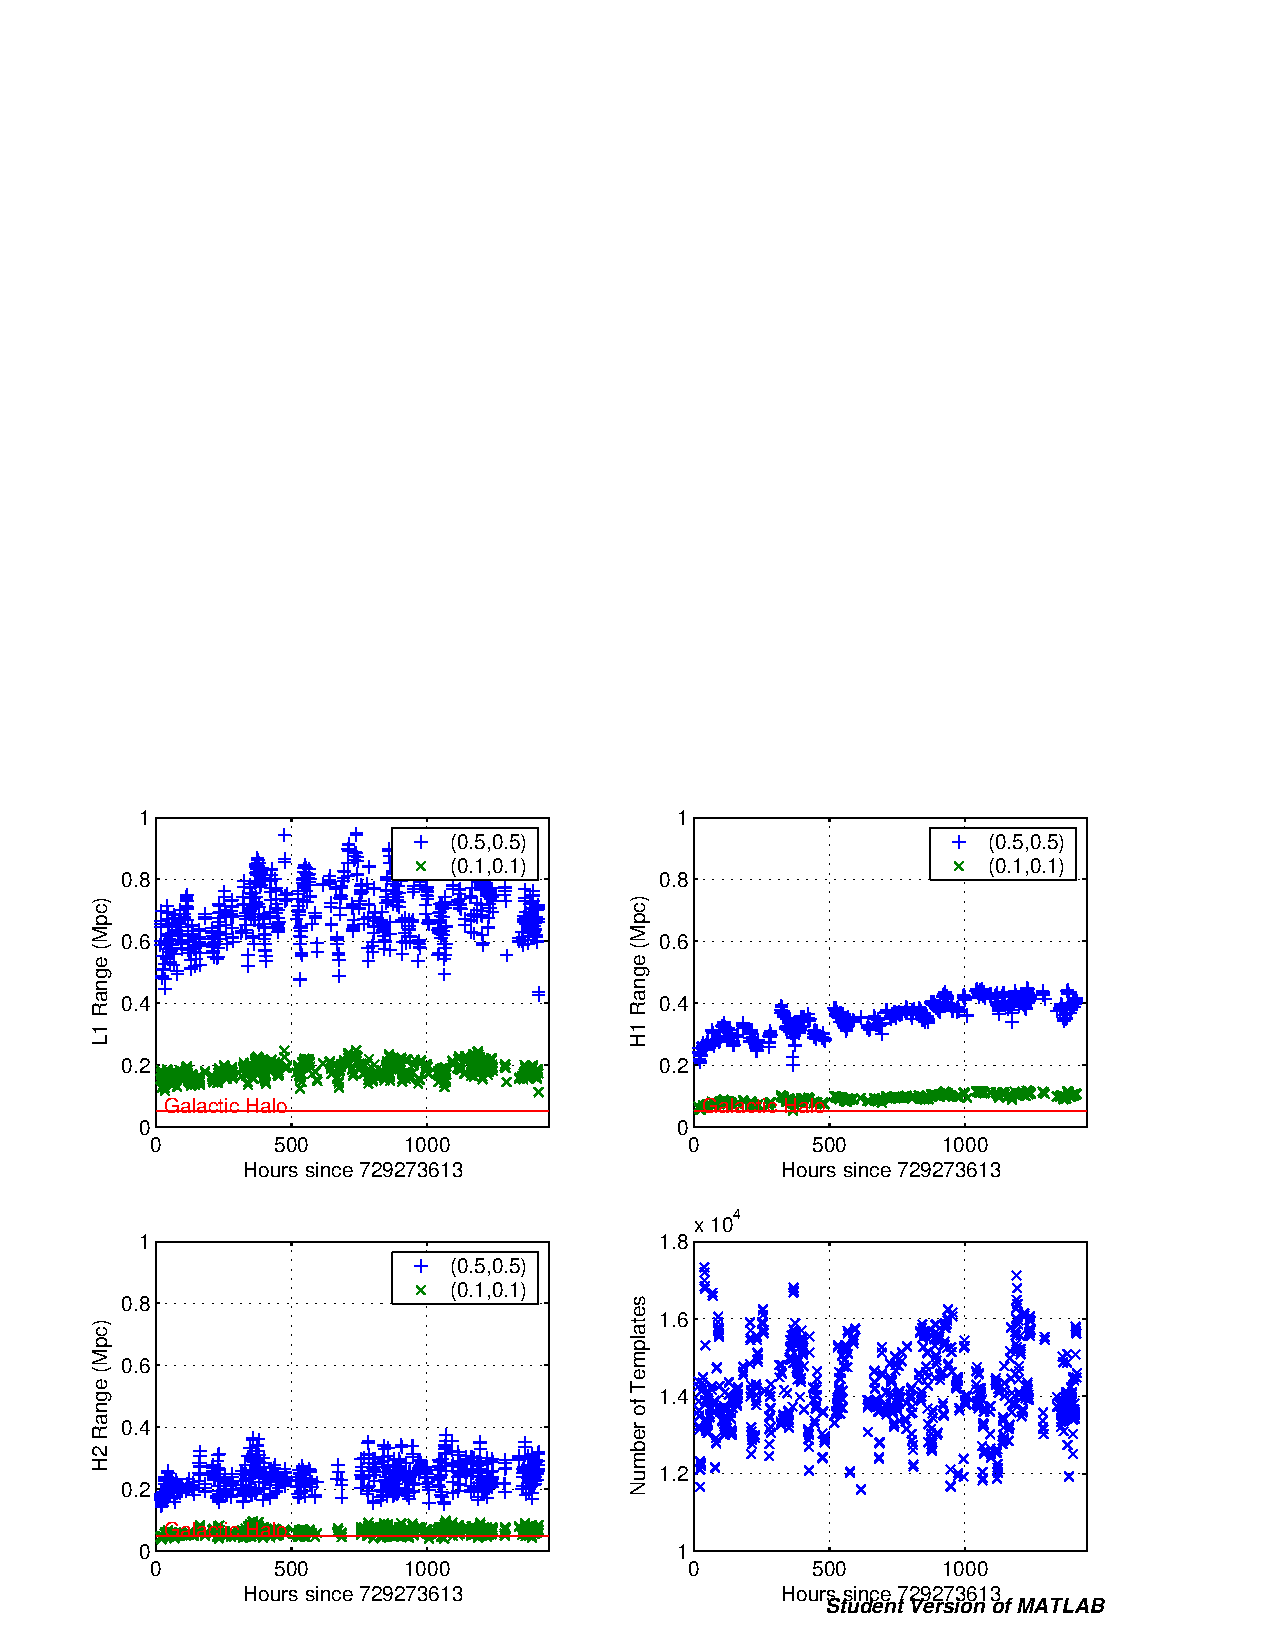
\includegraphics[width=\linewidth]{figures/result/s2_macho_range_summary}
\end{center}
\caption[S2 Interferometer Ranges and Template Bank Size]{%
\label{f:inspiral_summary}%
The bottom right plot shows the variation in the size of the MACHO search
template bank over the course of the S2 run. As described in the text, the
template bank is generated using L1 data to cover a region of parameter space
from $0.2\,M_\odot$ to $1.0\,M_\odot$ (component mass) at $95\%$ minimal
match. This template bank is used to filter the L1 data in the triggered
search pipeline. The other three plots show the variation in distance to which
the three LIGO interferometers can see an optimally oriented binary at
signal-to-noise ratio 8 over the S2 run. Since this is a function of the
masses of the binary, this range is shown for a $(0.1,0.1)\,M_\odot$ and a
$(0.5,0.5)\,M_\odot$ binary.
}
\end{figure}

\begin{figure}[p]
\begin{center}
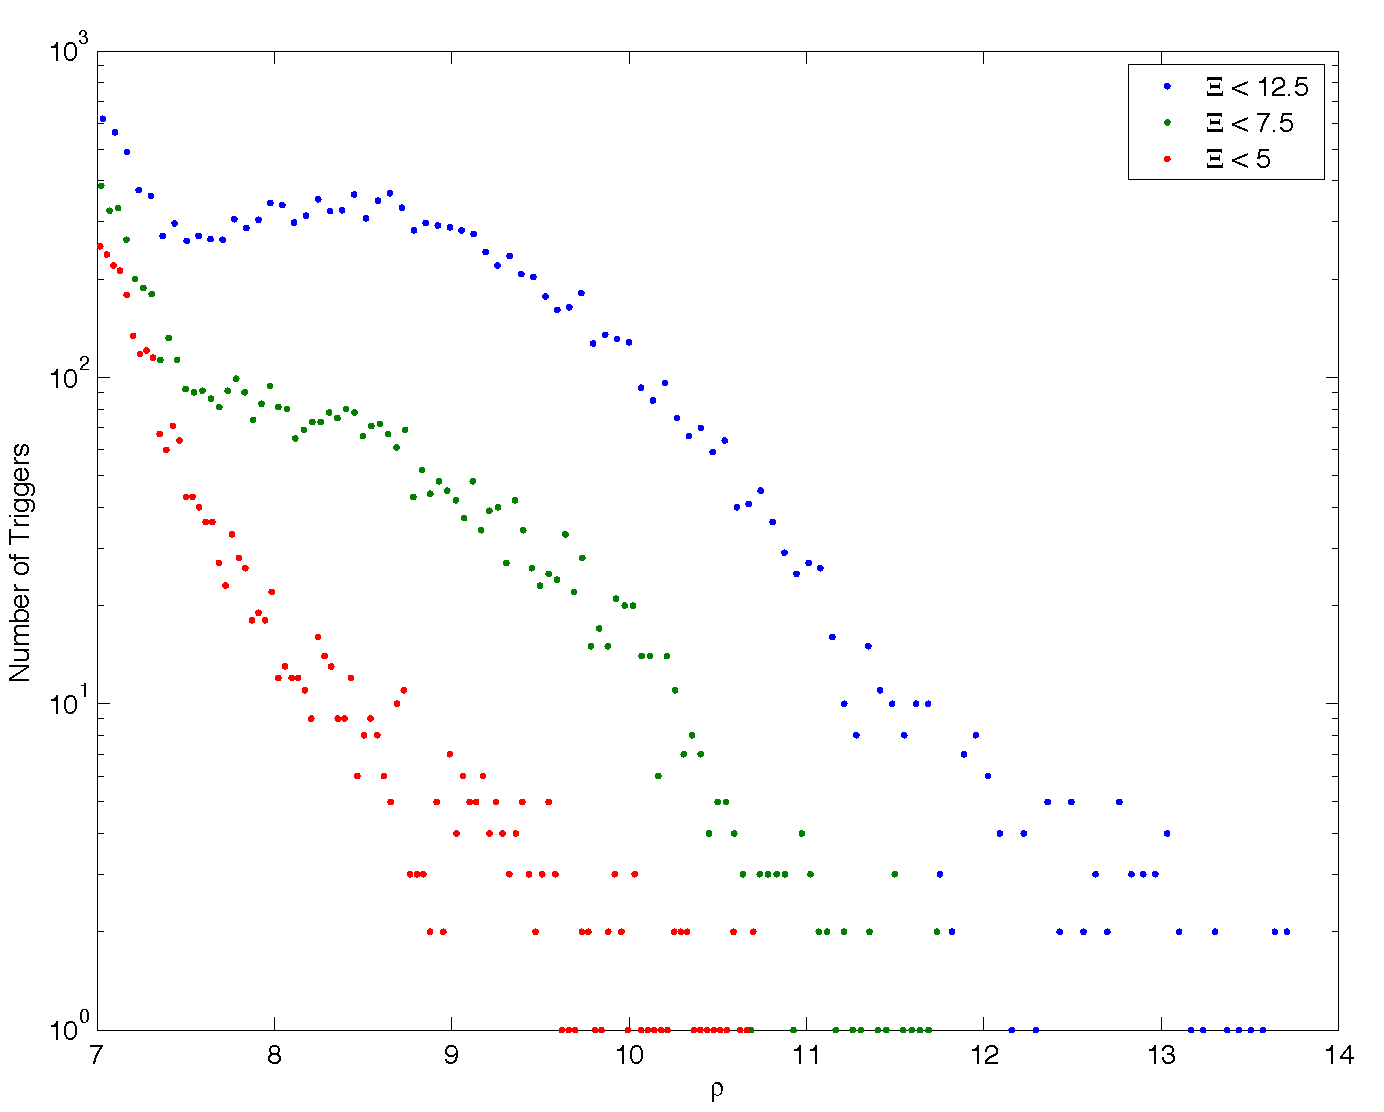
\includegraphics[width=\textwidth]{figures/result/h1l1_snr_hist_delta_0_04_chisq_12_5}
\end{center}
\caption[Tuning the $\chi^2$ Veto for H1]{%
\label{f:h1_chiqsq_tuning}%
The figure shows a histogram of all the triggers generated from the H1 data
using the triggered search (i.e. no coincidence with L1 or H2 has been applied
to the triggers). The signal-to-noise threshold is $\rho_\ast = 7$ and the
parameters of the $\chi^2$ veto are $p = 15, \delta^2 = 0.04, \Xi = 12.5$, as
in the S2 binary neutron star search. If the interferometer data is Gaussian,
then we would expect the histogram to be monotonically decreasing with
increasing signal-to-noise ratio; however, there is a pronounced ``hump'' in the
histogram at $\rho\approx 9$ suggesting some non-Gaussian feature in the data.
By lowering the value of $\Xi$ to $5$, we can remove this feature from the
histogram, but we must be careful in doing so that we do not reduce the
detection efficiency of the pipeline.
}
\end{figure}

\begin{figure}[p]
\begin{center}
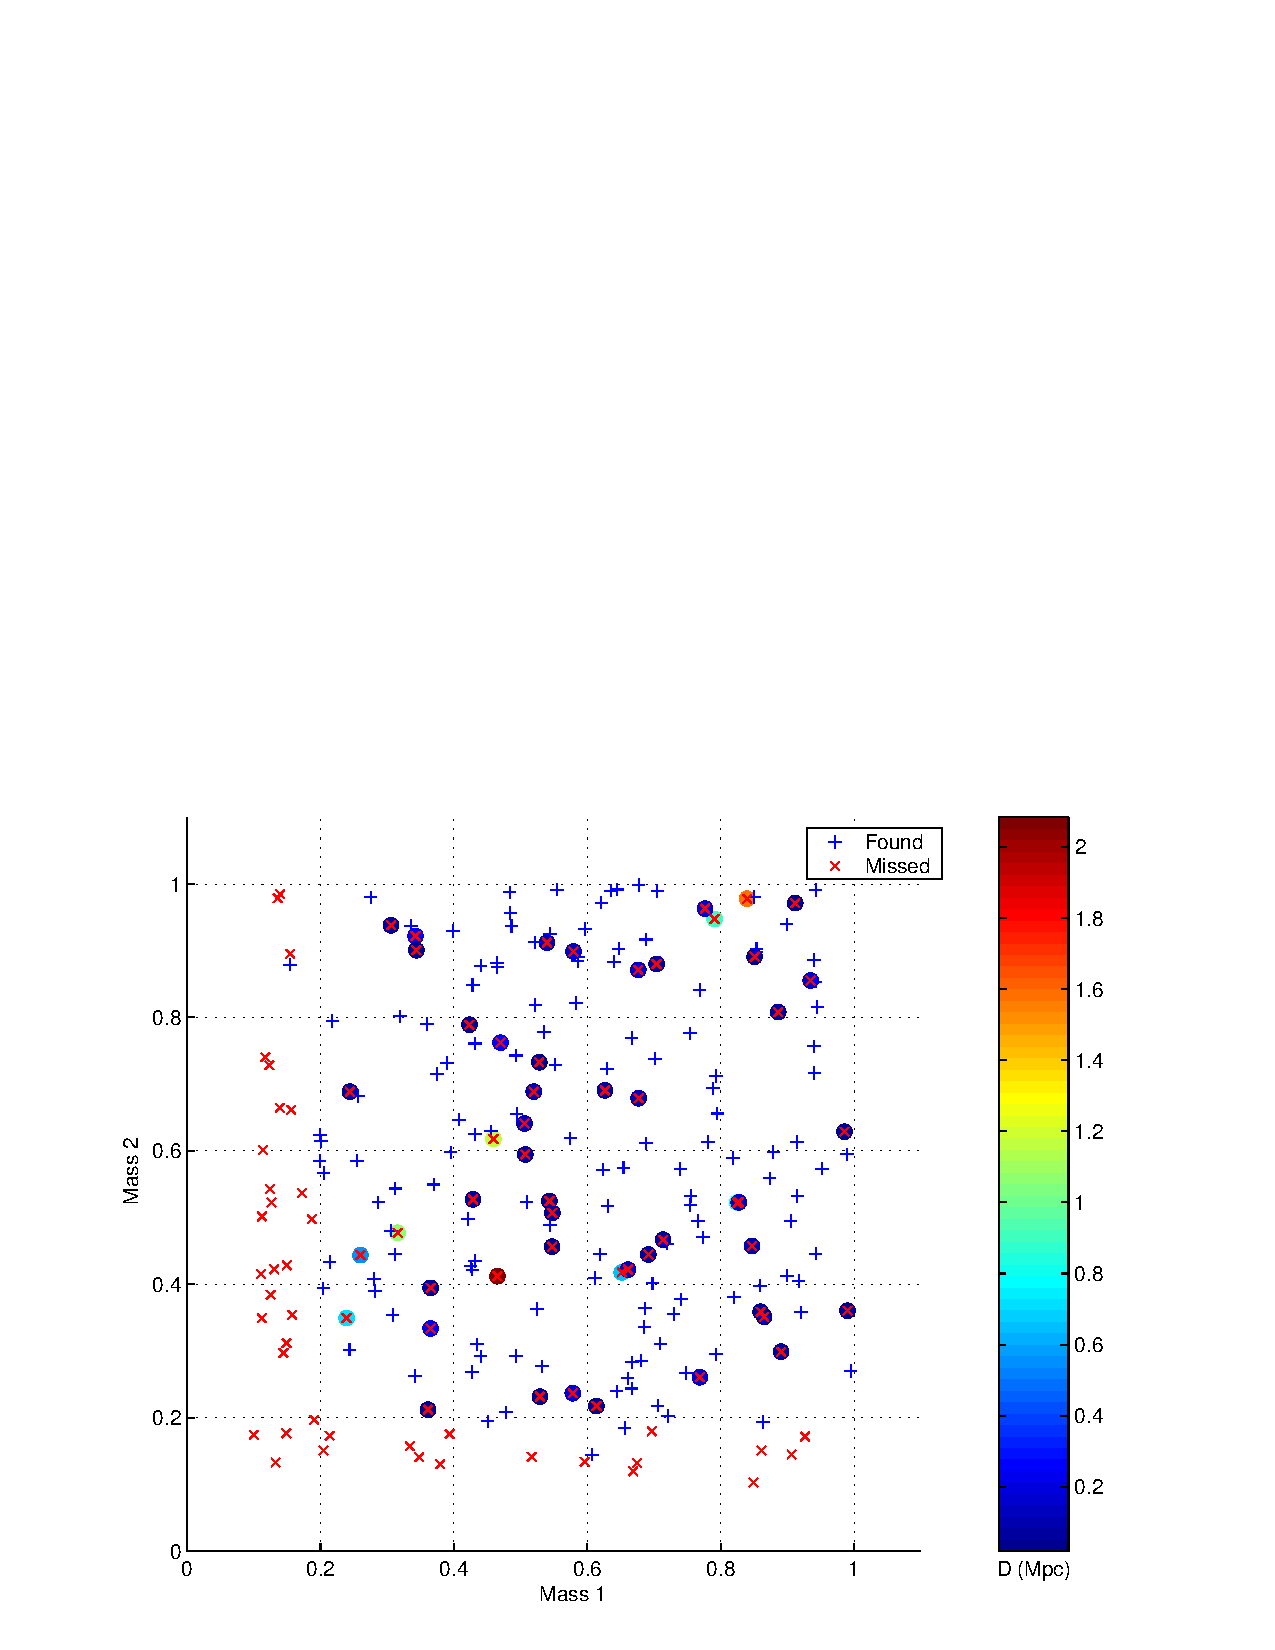
\includegraphics[width=\textwidth]{figures/result/h1_inj_mass_7_0_delta_0_04_chisq_12_5}
\end{center}
\caption[Found and Missed H1 Injections for $\Xi = 12.5 \delta^2 = 0.04$]{%
\label{f:h1_missed_tuning}%
The figure shows the results of a small Monte Carlo simulation used to test
the detection efficiency of the pipeline using H1 triggers (i.e. no
coincidence with L1 or H2 has been applied to the triggers). The
signal-to-noise threshold is $\rho_\ast = 7$ and the parameters of the
$\chi^2$ veto are $p = 15, \delta^2 = 0.04, \Xi = 12.5$. Found injections are
shown with a $+$, missed injections are shown with a $\times$ and the masses
of the injection are shown as the $x$ and $y$ coordinates. We would expect to
miss any injections with a mass component below $0.2\,M_\odot$ due to the
coverage of the template bank; however injections in the region inside the
bank should be detected, unless they are at an effective distance larger than
the range of the interferometer. The missed injections that we would expect to
find are color coded according to the effective distance at which they are
injected.  Several injections are missed as they are at a large effective
distance (e.g.  the injection at $(0.48,0.42)\,M_\odot$); however there are
may missed injections at distances $< 200$~kpc which should be detectable in
the H1 data (e.g. the injection at $(0.88,0.91)\,M_\odot$). Investigation of
the missed injections showed they had large values of signal-to-noise ratio,
but were vetoed by the $\chi^2$ test. This suggests that the search parameters
used must be re-tuned to increase the detection efficiency.
}
\end{figure}

\begin{figure}[p]
\begin{center}
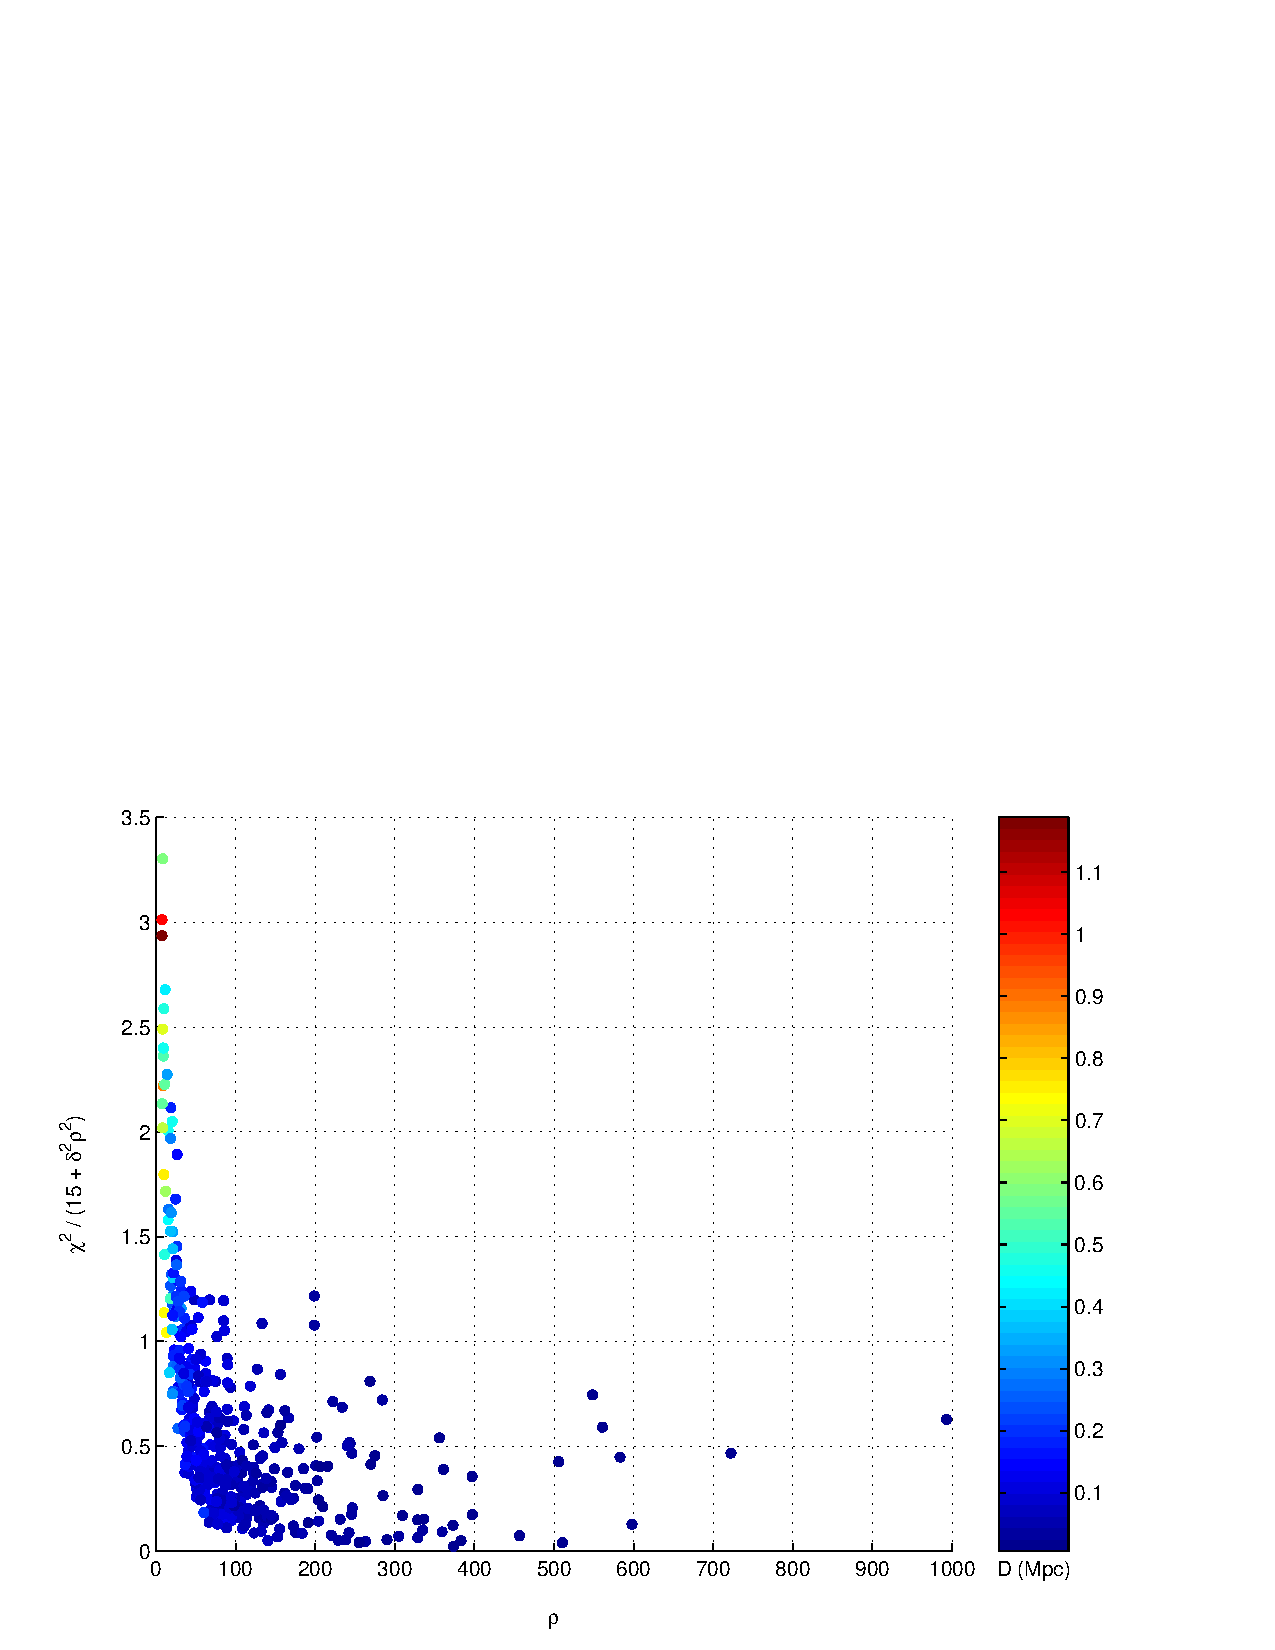
\includegraphics[width=0.7\textwidth]{figures/result/l1_inj_snr_7_0_delta_0_04_chisq_5_0}\\
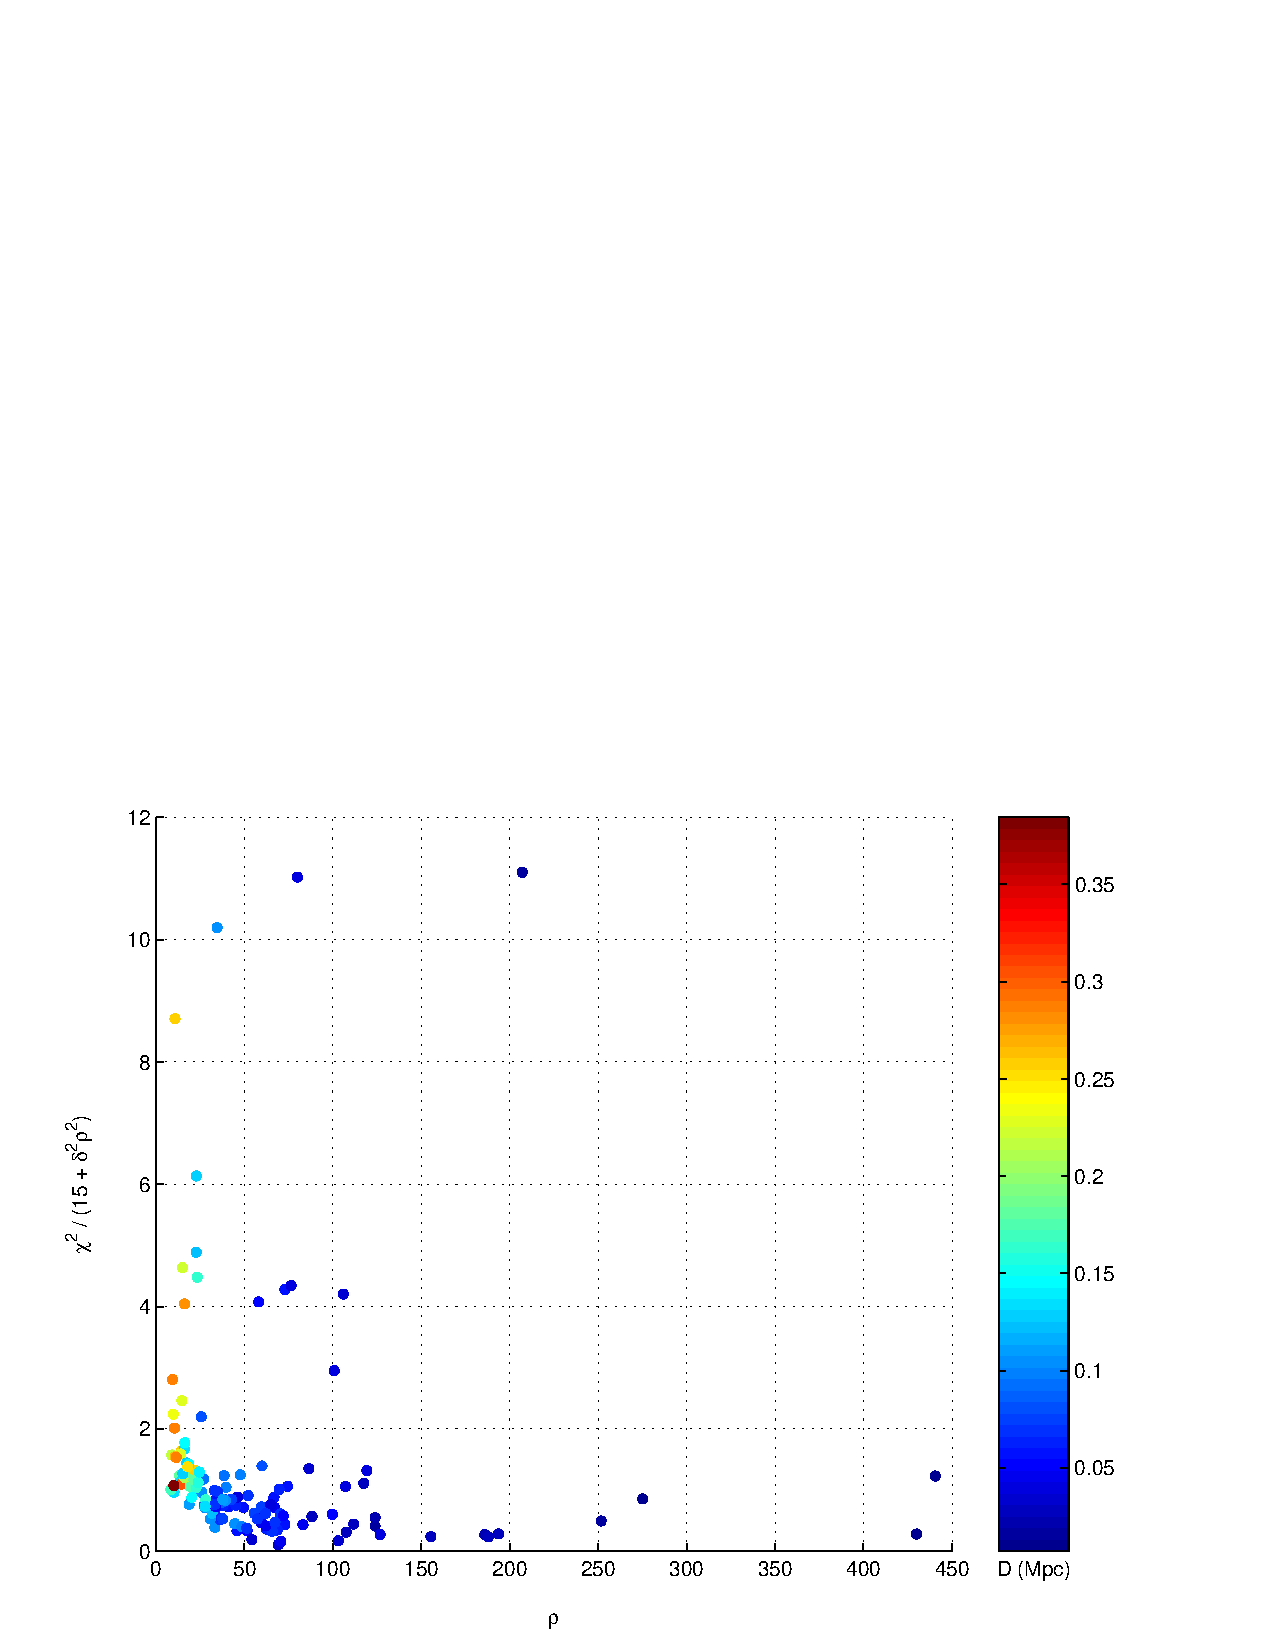
\includegraphics[width=0.7\textwidth]{figures/result/h1_inj_snr_7_0_delta_0_04_chisq_12_5}
\end{center}
\caption[Illustration of Tuning Based on Injections]{%
\label{f:h1_inj_xi_tuning}%
The plots in this figure show the values of $\rho$ and $\Xi = \chi^2/(15 +
\delta^2\rho^2)$ for the inspiral triggers corresponding to injected signals
found by the triggered search pipeline. The upper plot shows L1 triggers and
the lower plot shows H1 triggers (which correspond to the found injections of
figure \ref{f:h1_missed_tuning}). No coincidence has been applied to the H1
triggers at this stage; however they are generated using template banks
produced from L1 triggers. The color of each trigger shows the effective
distance at which it was injected.  Both plots are generated with a
signal-to-noise threshold of $\rho_\ast = 7$, and the parameters of the
$\chi^2$ veto were $p = 15, \delta^2 = 0.04$ and $\Xi_\mathrm{L1} = 12.5,
\Xi_\mathrm{L1} = 5.0$, values chosen based on the tuning of the S2 binary
neutron star search. It can be seen that, at a given signal-to-noise ratio,
the H1 triggers typically have higher values of $\Xi$ than the L1 triggers.
This is due to the a larger mismatch between the injected signal and the
templates in the H1 triggered bank.
}
\end{figure}

\begin{figure}[p]
\begin{center}
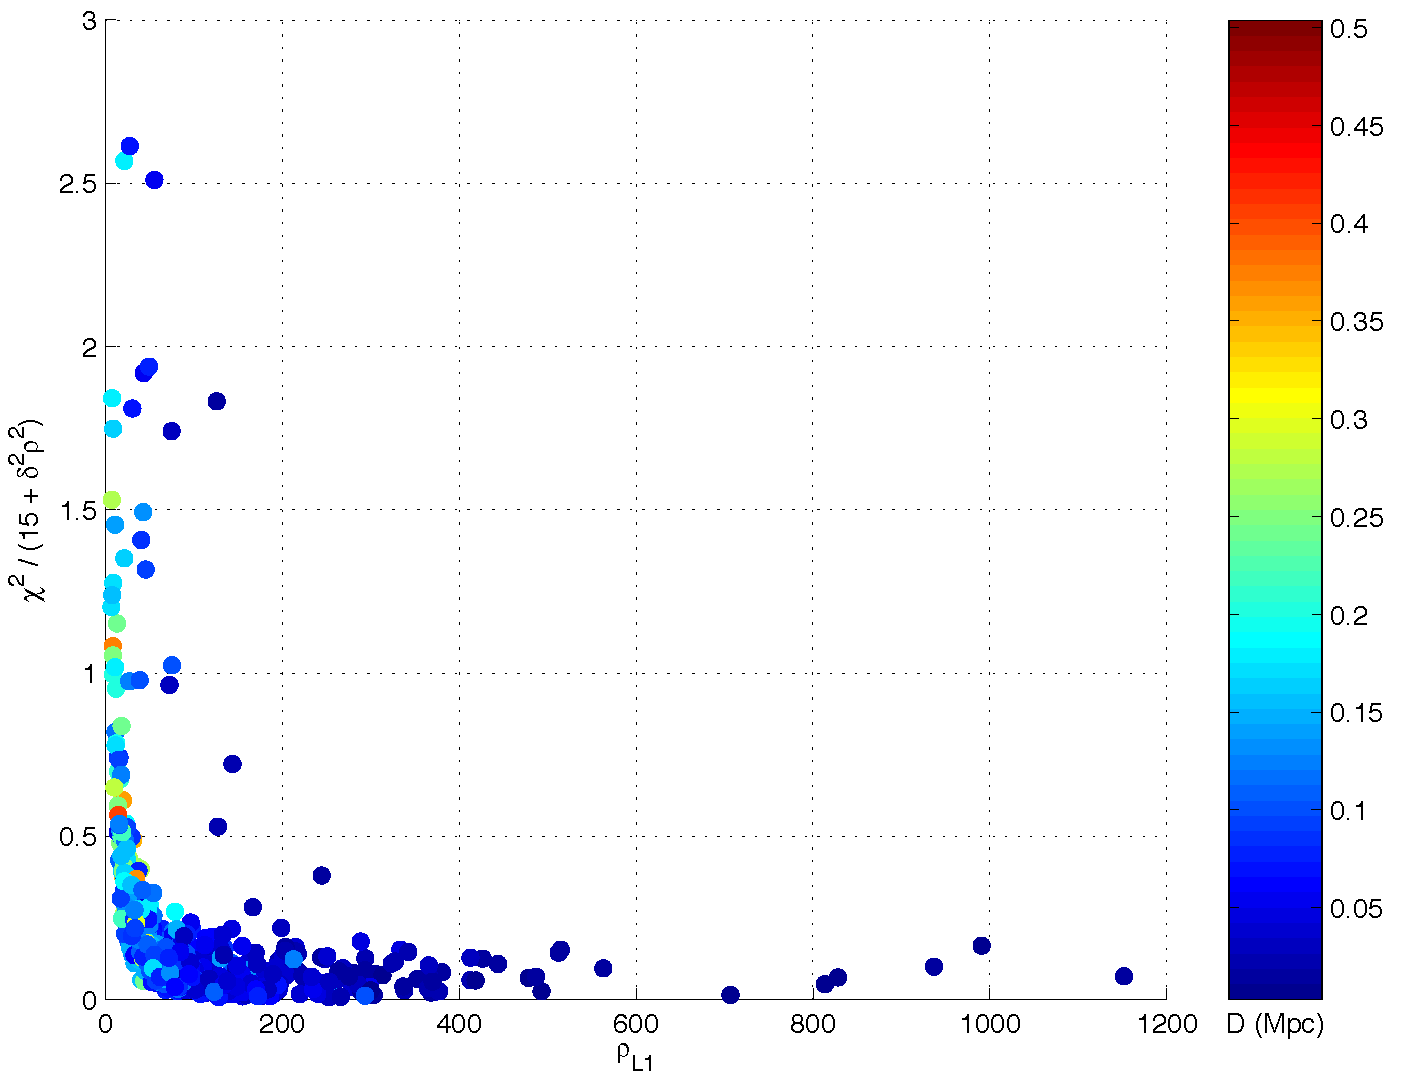
\includegraphics[width=0.7\textwidth]{figures/result/l1_inj_snr_final}\\
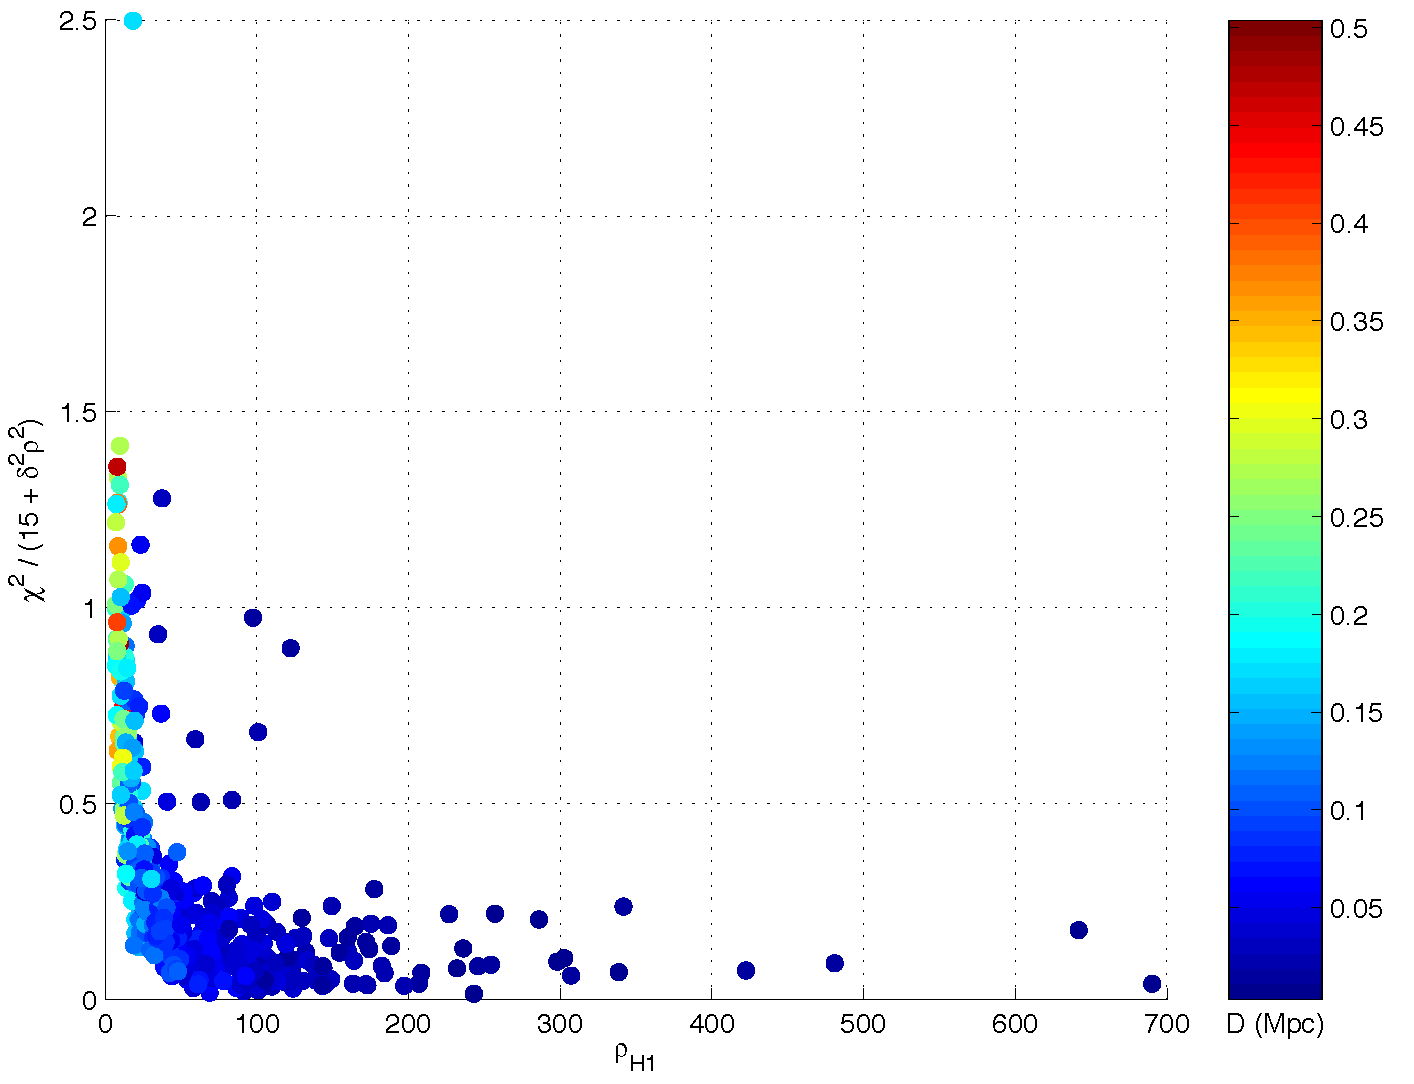
\includegraphics[width=0.7\textwidth]{figures/result/h1_inj_snr_final}
\end{center}
\caption[Signal-to-noise ratio and $\chi^2$-veto for Injected Signals]{%
\label{f:h1_inj_xi_final}%
The plots in this figure should show the observed values of $\rho$ and $\Xi
= \chi^2/(15 + \delta^2\rho^2)$ for the inspiral triggers corresponding to
injected signals found by the triggered search pipeline using the final set of
parameters chosen. The upper plot shows L1 triggers and the lower plot shows
H1 triggers. No coincidence has been applied to the H1 triggers at this stage;
however they are generated using template banks produced from L1 triggers.
These plots should be compared to those shown in
figure~\ref{f:h1_inj_xi_tuning}. By tuning the value of $\delta^2$ to $0.2$,
it can be seen that much lower values of $\Xi$ are obtained for the H1
injections. This suggests that we could further reduce the threshold
$\Xi_\ast$, although this was not done as no coincident triggers were found in
the playground data and a looser value of $\delta$ allowed us to probe the
region slightly outside the template bank parameter space.
}
\end{figure}

\begin{table}[p]
\begin{tabular}{cllr}
Parameter & Description  & value \\
\hline 
$f_\mathrm{hp}$ & High Pass Filter Frequency  & $100$~Hz \\
$O_\mathrm{hp}$ & High Pass Filter Order  & $100$~Hz \\
$f_\mathrm{low}$ & Low Frequency Cutoff  & $100$~Hz \\
$m_\mathrm{min}$ & Template bank lower component mass  & $0.2\,M_\odot$ \\
$m_\mathrm{max}$ & Template bank upper component mass  & $1.0\,M_\odot$ \\
$\mathbb{M}$ & L1 template bank minimal match  & 0.95 \\
$\rho^\ast_\mathrm{L1}$ & L1 signal-to-noise ratio threshold & 7.0 \\
$\Xi^\ast_\mathrm{L1}$ & L1 $\chi^2$ veto threshold & 3.1 \\
$\rho^\ast_\mathrm{H1}$ & H1 signal-to-noise ratio threshold & 7.0 \\
$\Xi^\ast_\mathrm{H1}$ & H1 $\chi^2$ veto threshold & 5.0 \\
$\rho^\ast_\mathrm{H2}$ & H2 signal-to-noise ratio threshold & 7.0 \\
$\Xi^\ast_\mathrm{H2}$ & H2 $\chi^2$ veto threshold & 10.0 \\
$p$ & Number of bins in $\chi^2$ veto & 15 \\
$\delta^2$ & $\chi^2$ veto mismatch parameter & 0.2 \\
$\delta m$ & Trigger mass coincidence parameter & 0.0 \\
$\delta t_\mathrm{HH}$ & H1-H2 trigger time coincidence parameter & 0.001 s \\
$\delta t_\mathrm{LH}$ & L1-H1, L1-H2 trigger time coincidence parameter & 0.011 s \\
$\kappa_{HH}$ & H1-H2 trigger amplitude coincidence parameter & 0.5 \\
$\kappa_{LH}$ & L1-H1, L1-H2 trigger amplitude coincidence parameter & 1000.0 \\
$\epsilon$ & Trigger amplitude coincidence parameter & 2.0
\end{tabular}
\caption[Pipeline Parameters used in S2 BBHMACHO Search]{%
\label{t:ifo_params}%
A complete list of the parameters that were selected at the various
stages of the pipeline. These values are justified in the text.
}
\end{table}

\begin{figure}[p]
\begin{center}
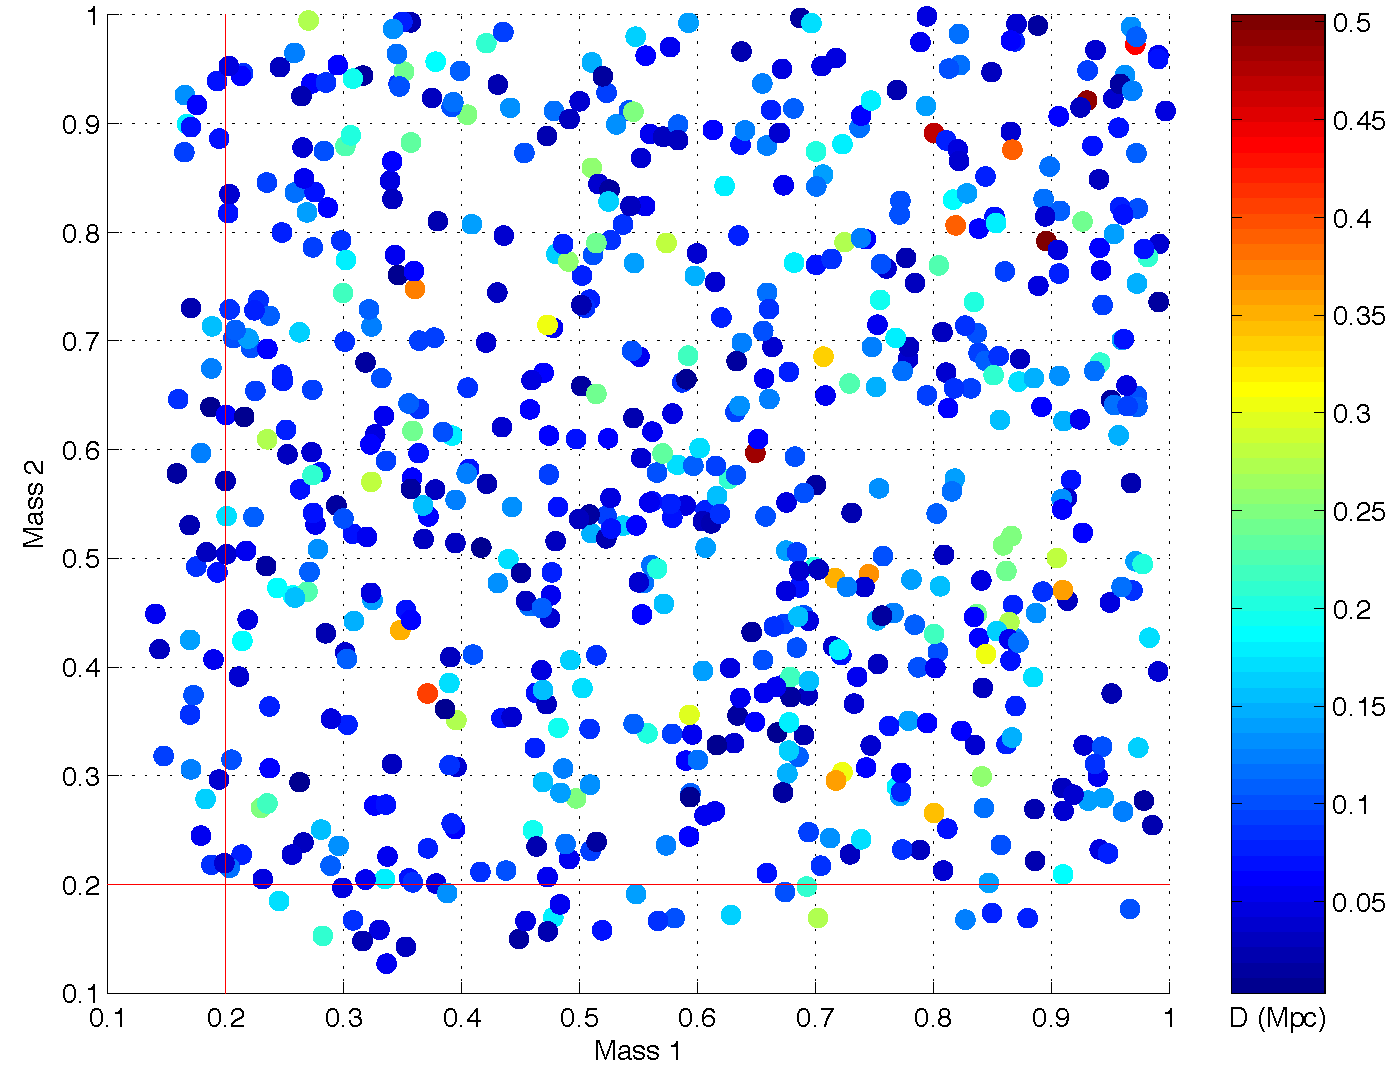
\includegraphics[width=0.7\textwidth]{figures/result/m1m2_found}\\
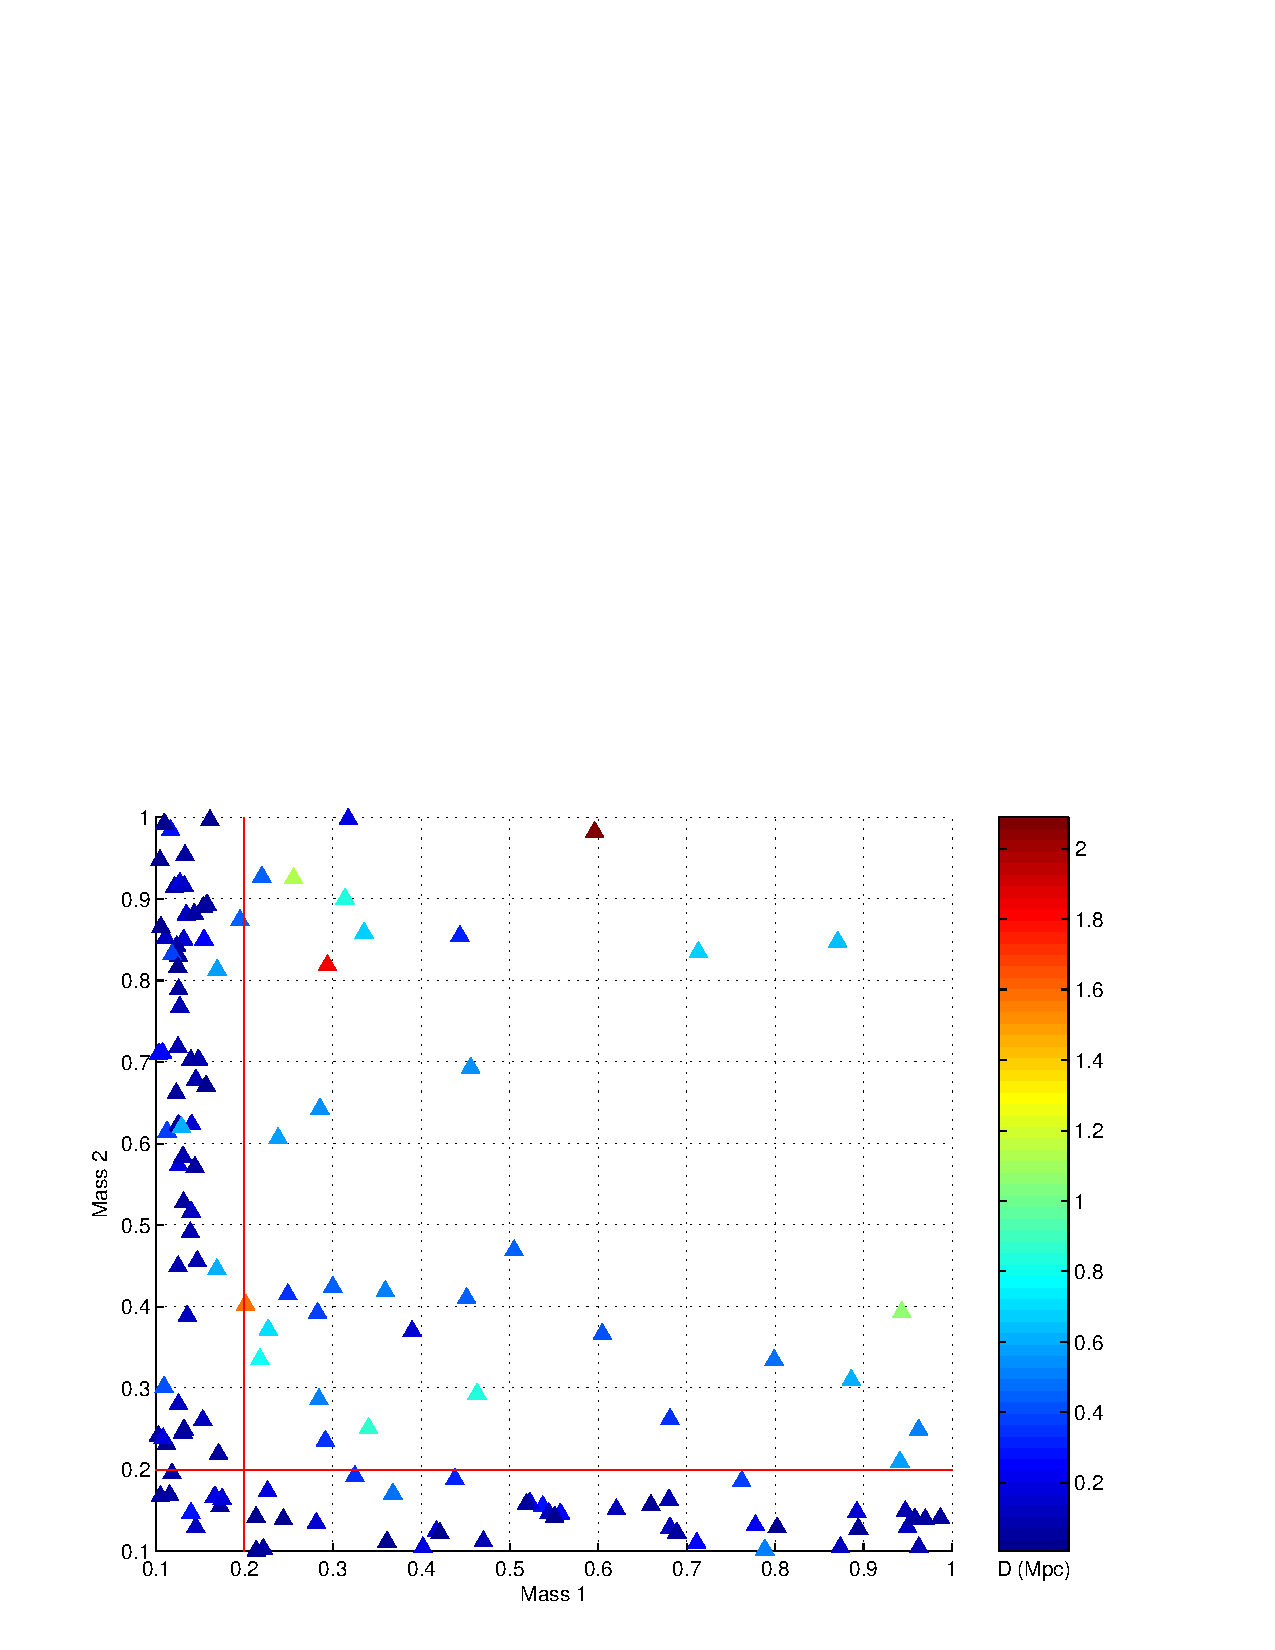
\includegraphics[width=0.7\textwidth]{figures/result/m1m2_missed}
\end{center}
\caption[Injections Detected and Missed by Monte Carlo Simulation]{%
\label{f:m1m2_found_missed}%
This figure shows the results of the Monte Carlo simulation used to measure
the efficiency of the pipeline once parameter tuning had been completed; these
detected triggers have survived all threshold and coincidence tests.  The
injections that are detected are shown as circles on the upper plot.  The
lower plot shows the injections that were not detected: stars correspond to
missed injections in the triple coincident data, upward pointing triangles to
the L1-H1 data and downward pointing triangles to the L1-H2 data. The $x$ and
$y$ coordinates are the mass parameters $m_1$ and $m_2$ of each injection,
respectively. The color of each injection represents the effective distance in
the Hanford interferometers at which the waveform was injected (since the LHO
interferometers limit the sensitivity of the search).  The horizontal and
vertical red lines show the edge of the template bank parameter space. 
%Notice
%that the effective distance of missed injections inside the bank space are
%consistent with the ranges of the interferometers. We can also see that by
%loosening the value of $\delta$ we have been able to search for injections
%outside the parameter to a value of $\sim 0.15\,M_\odot$, the lower limit
%suggested by microlensing observations.
}
\end{figure}

\begin{figure}[p]
\begin{center}
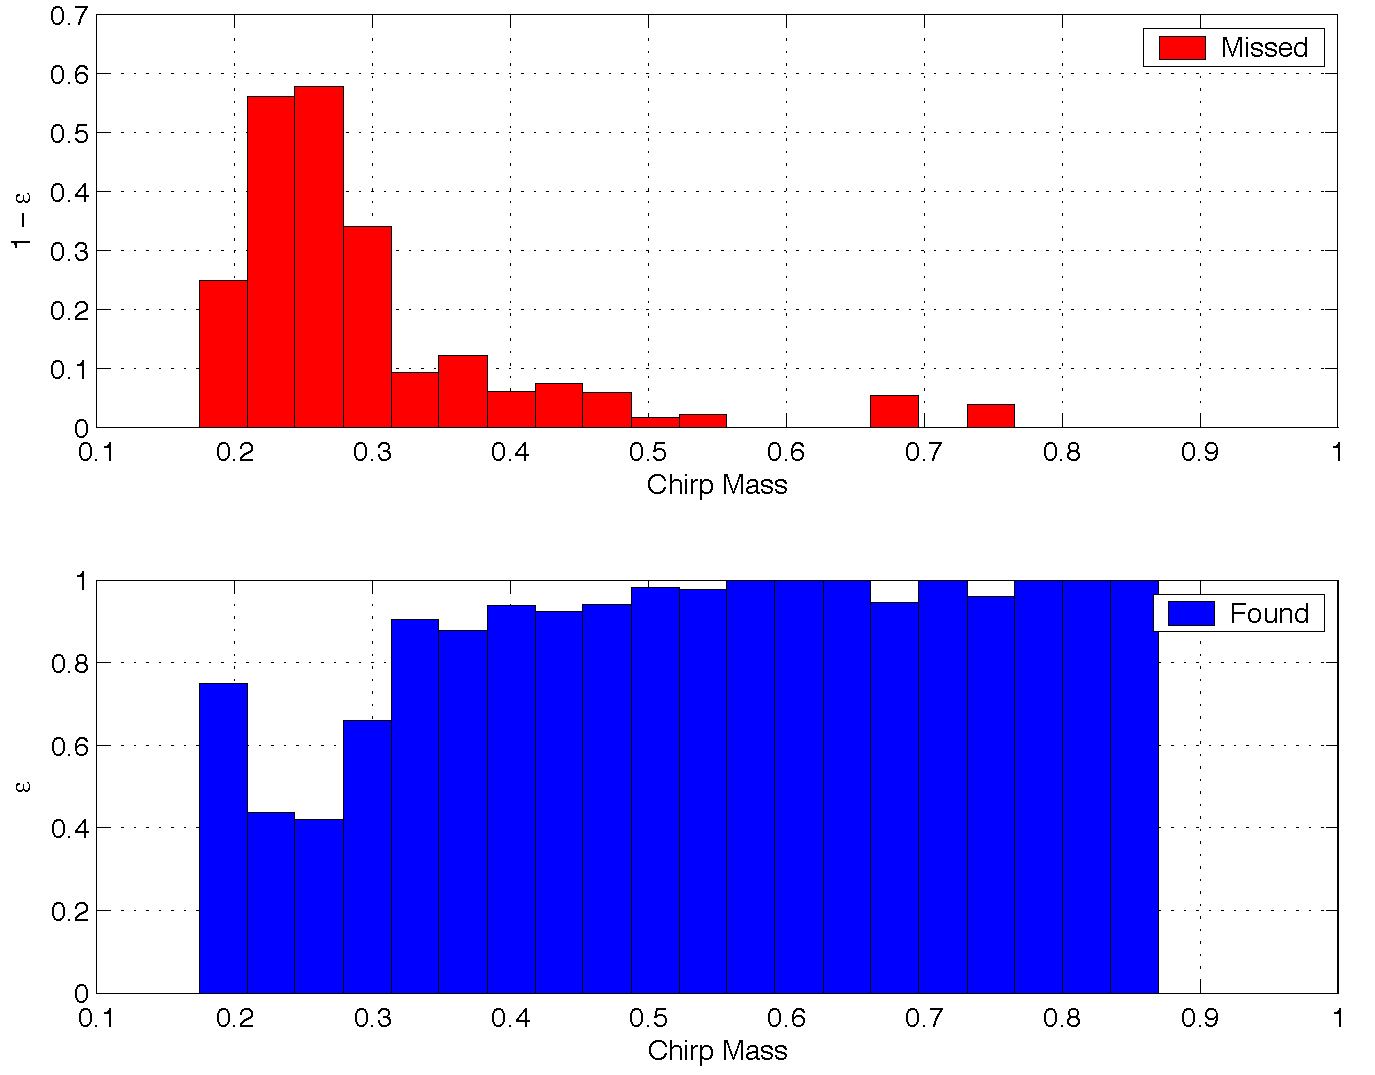
\includegraphics[width=0.7\textwidth]{figures/result/mchirp_eff} \\
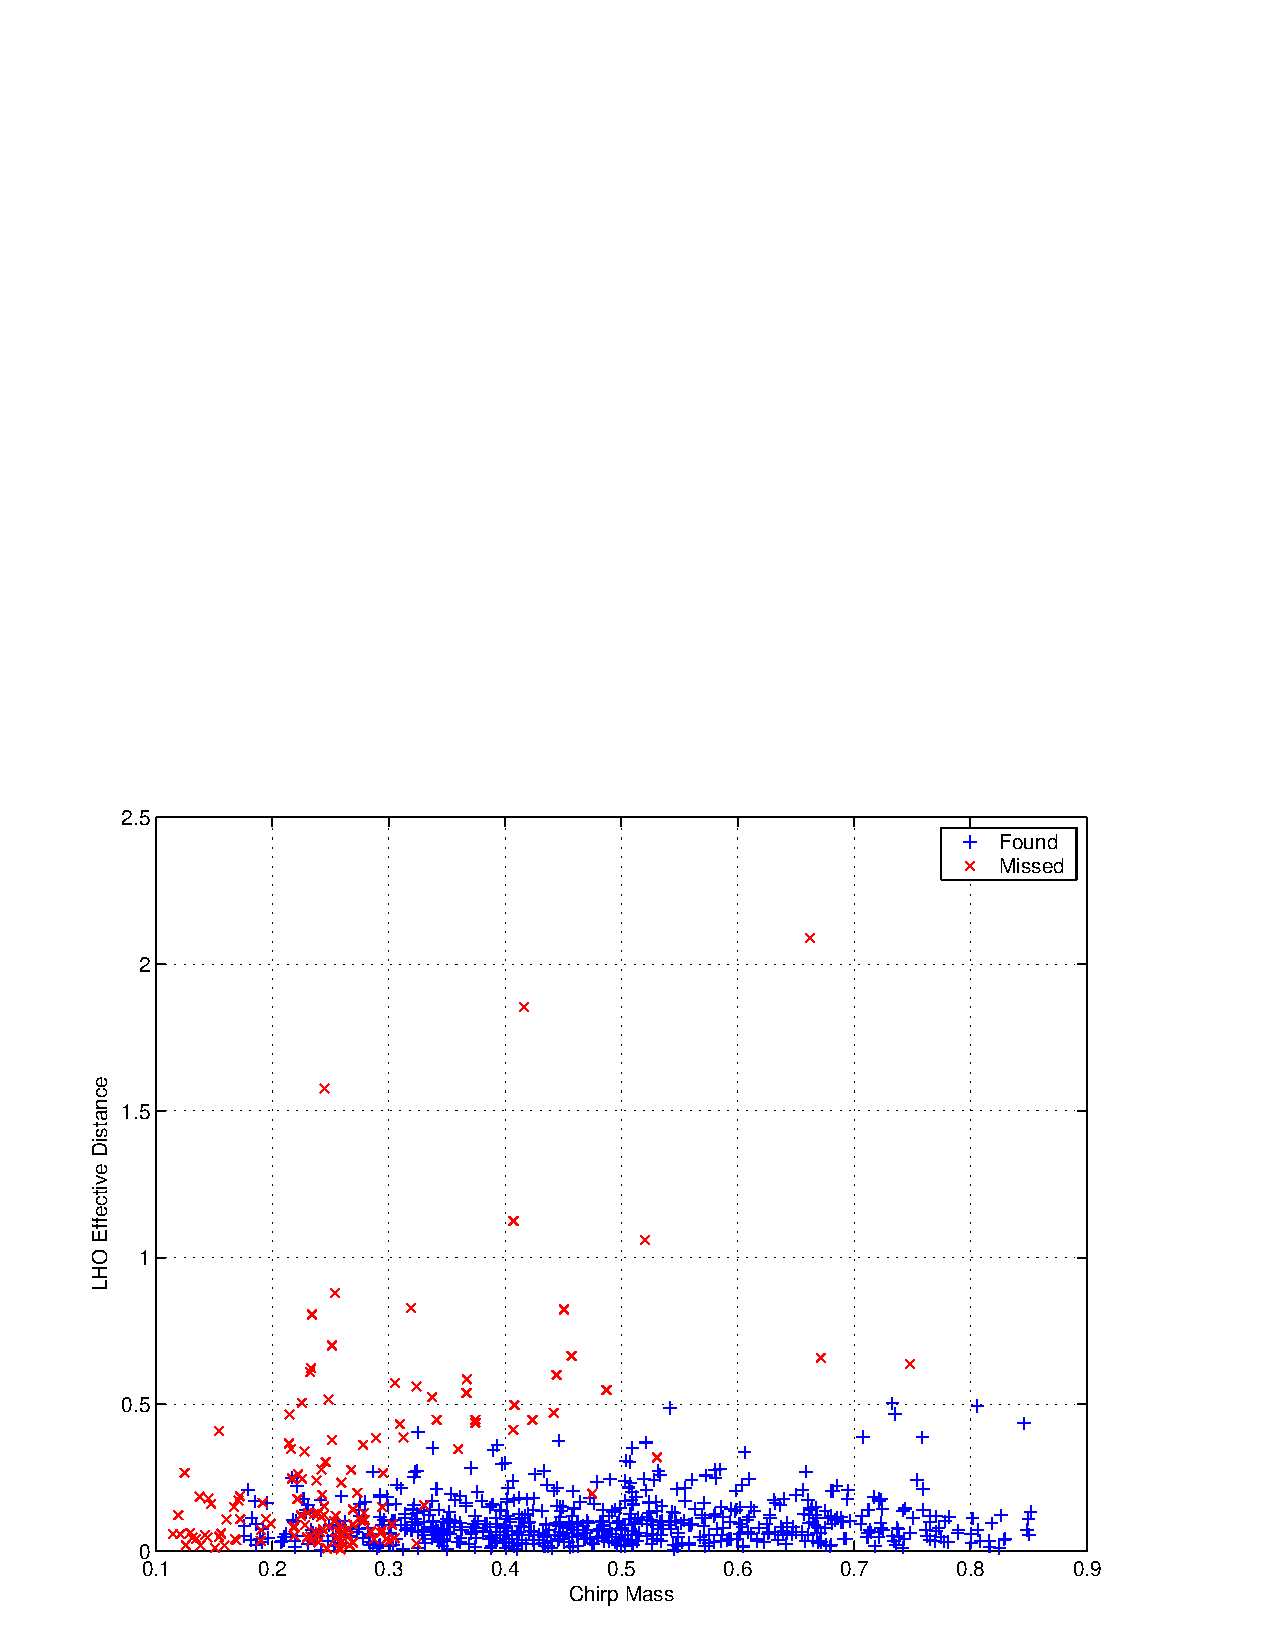
\includegraphics[width=0.7\textwidth]{figures/result/mchirp_found_missed}
\end{center}
\caption[Search Efficiency as a Function of Chirp Mass]{%
\label{f:mchirp_eff}%
The upper two plots show the efficiency of the pipeline $\varepsilon$ and the
loss of the search $1-\varepsilon$ as a function of the injected signal chirp
mass $\mathcal{M}$ measured by the Monte Carlo Simulation. The lower plot
shows the chirp mass and effective distance in LHO of the injections used to
measure the pipeline efficiency; detected injections are shown with a $+$ and
missed injections are shown with a $\times$. It can be seen that the
efficiency of the pipeline is unity very close to unity for high values of
$\mathcal{M}$ and falls as the chirp mass decreases. There appears to be an
anomalously large value of $\varepsilon$ at $\mathcal{M}\approx 0.18$, however
it can be seen from the lower plot that there were comparatively few
injections at this chirp mass, so this may be an effect of small number
statistics. Further Monte Carlo simulations will be able to test this
hypothesis.
}
\end{figure}

\begin{figure}[p]
\begin{center}
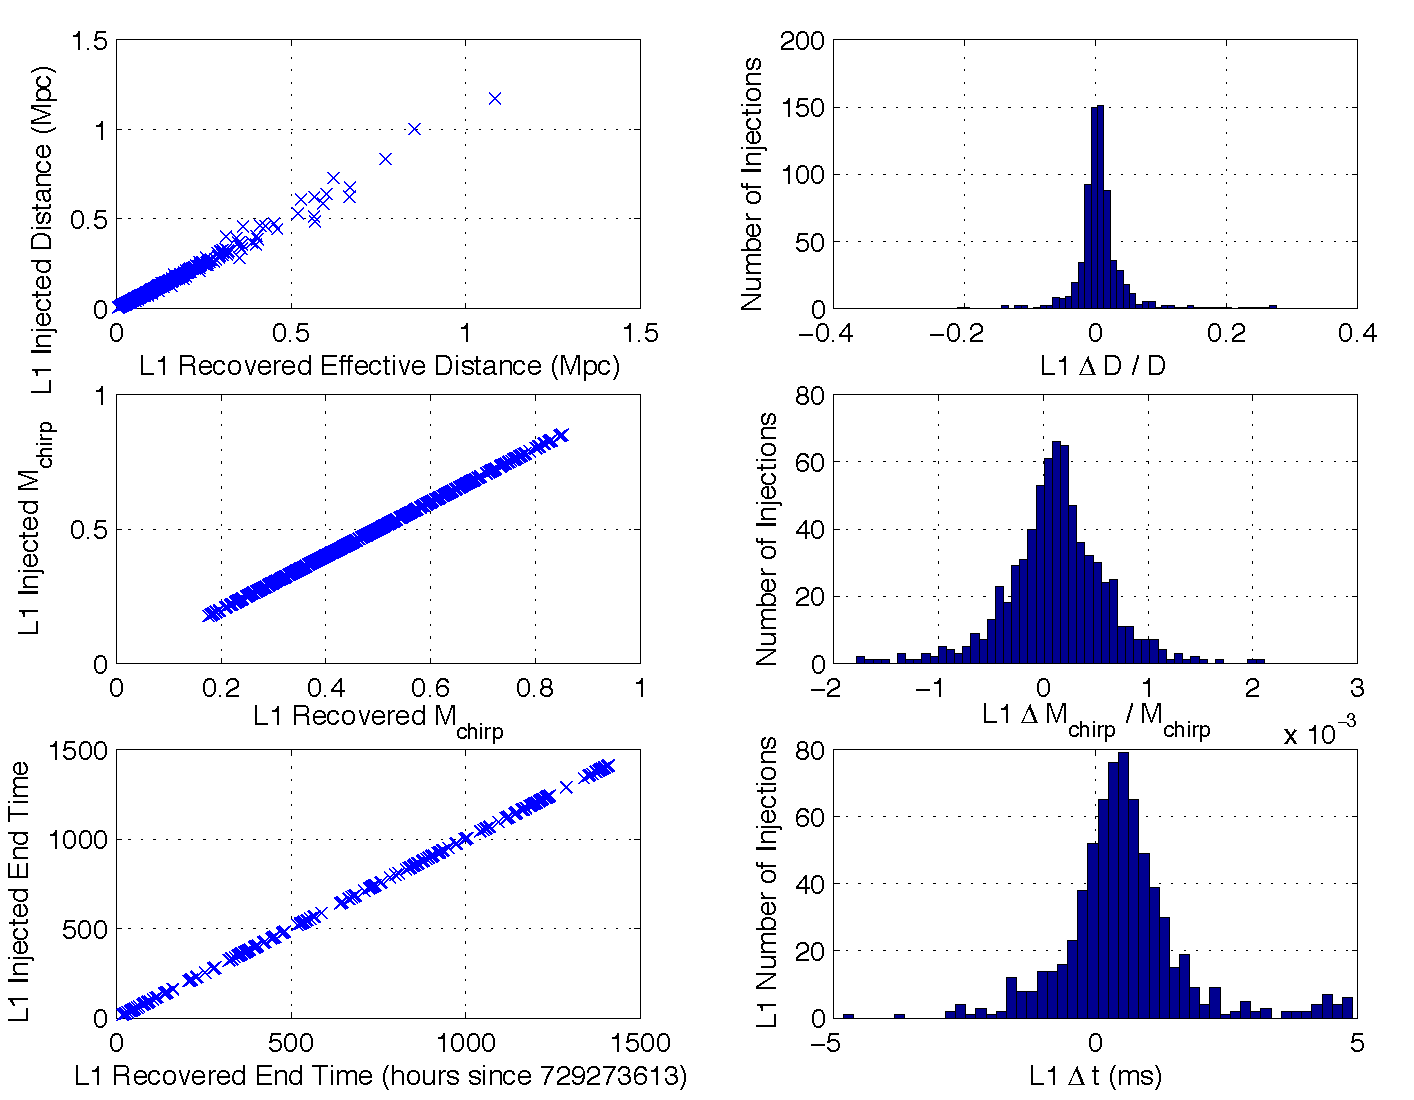
\includegraphics[width=\textwidth]{figures/result/l1_param_error}
\end{center}
\caption[Measurement accuracy of L1 Injection Parameters]{%
\label{f:l1_param_error}%
The panels in this figure compare the measured values of effective distance,
chirp mass and end time with the known values for the injected waveforms in
the Monte Carlo simulation in the L1 detector.
}
\end{figure}

\begin{figure}[p]
\begin{center}
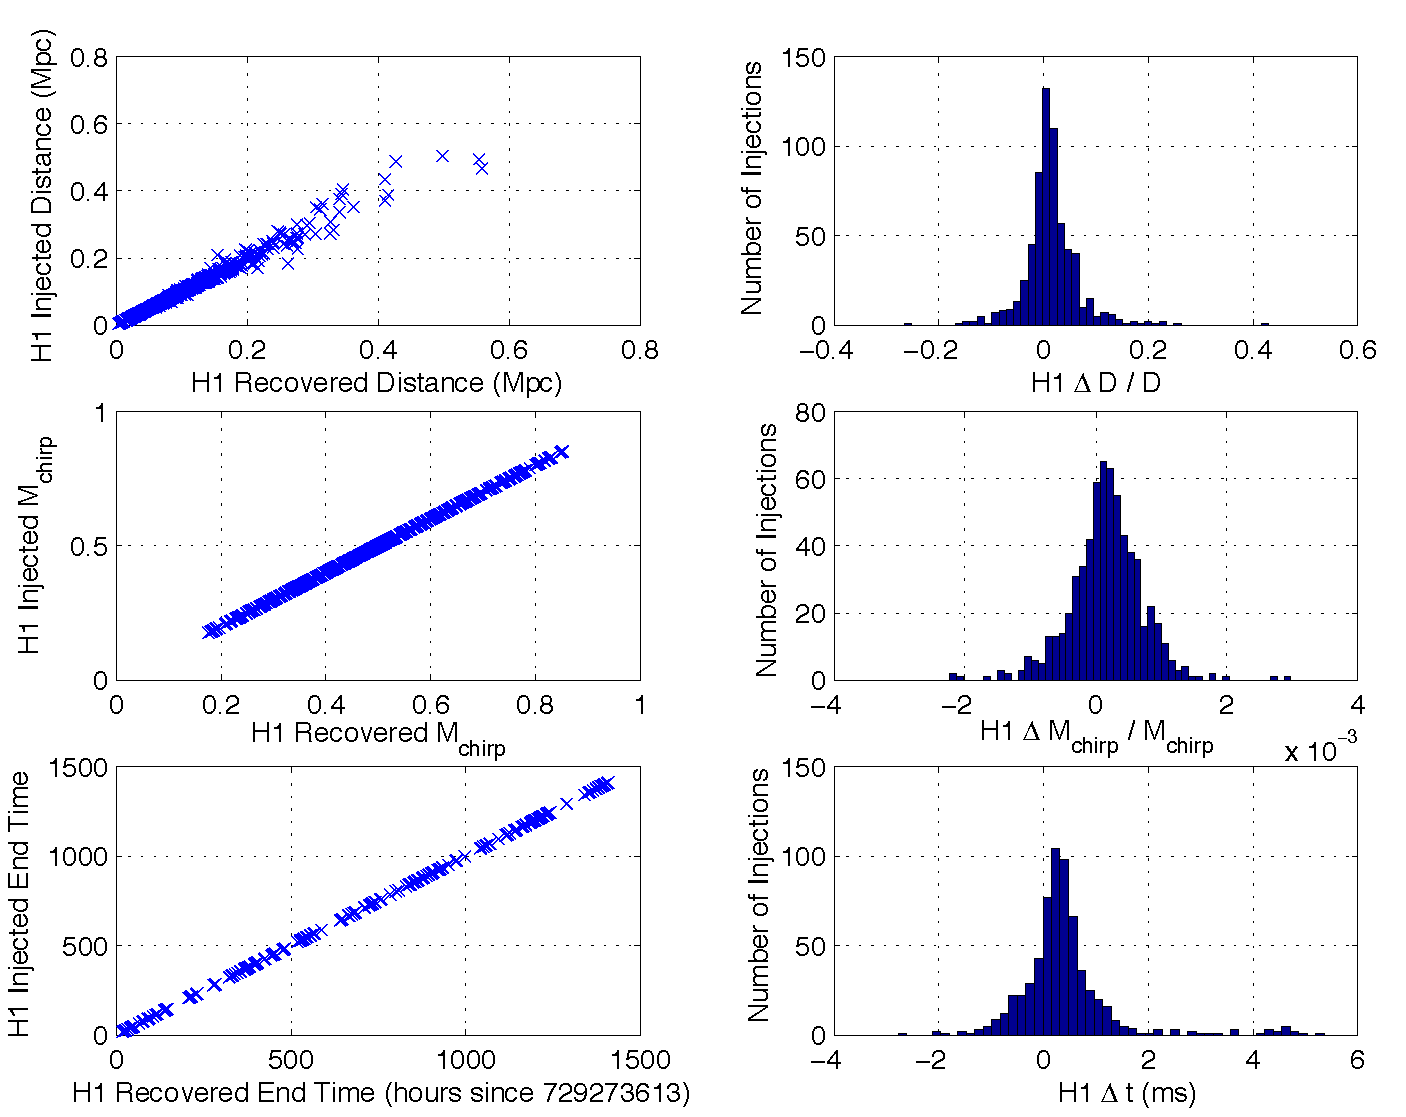
\includegraphics[width=\textwidth]{figures/result/h1_param_error}
\end{center}
\caption[Measurement accuracy of H1 Injection Parameters]{%
\label{f:h1_param_error}%
The panels in this figure compare the measured values of effective distance,
chirp mass and end time with the known values for the injected waveforms in
the Monte Carlo simulation in the H1 detector.
}
\end{figure}

\begin{figure}[p]
\begin{center}
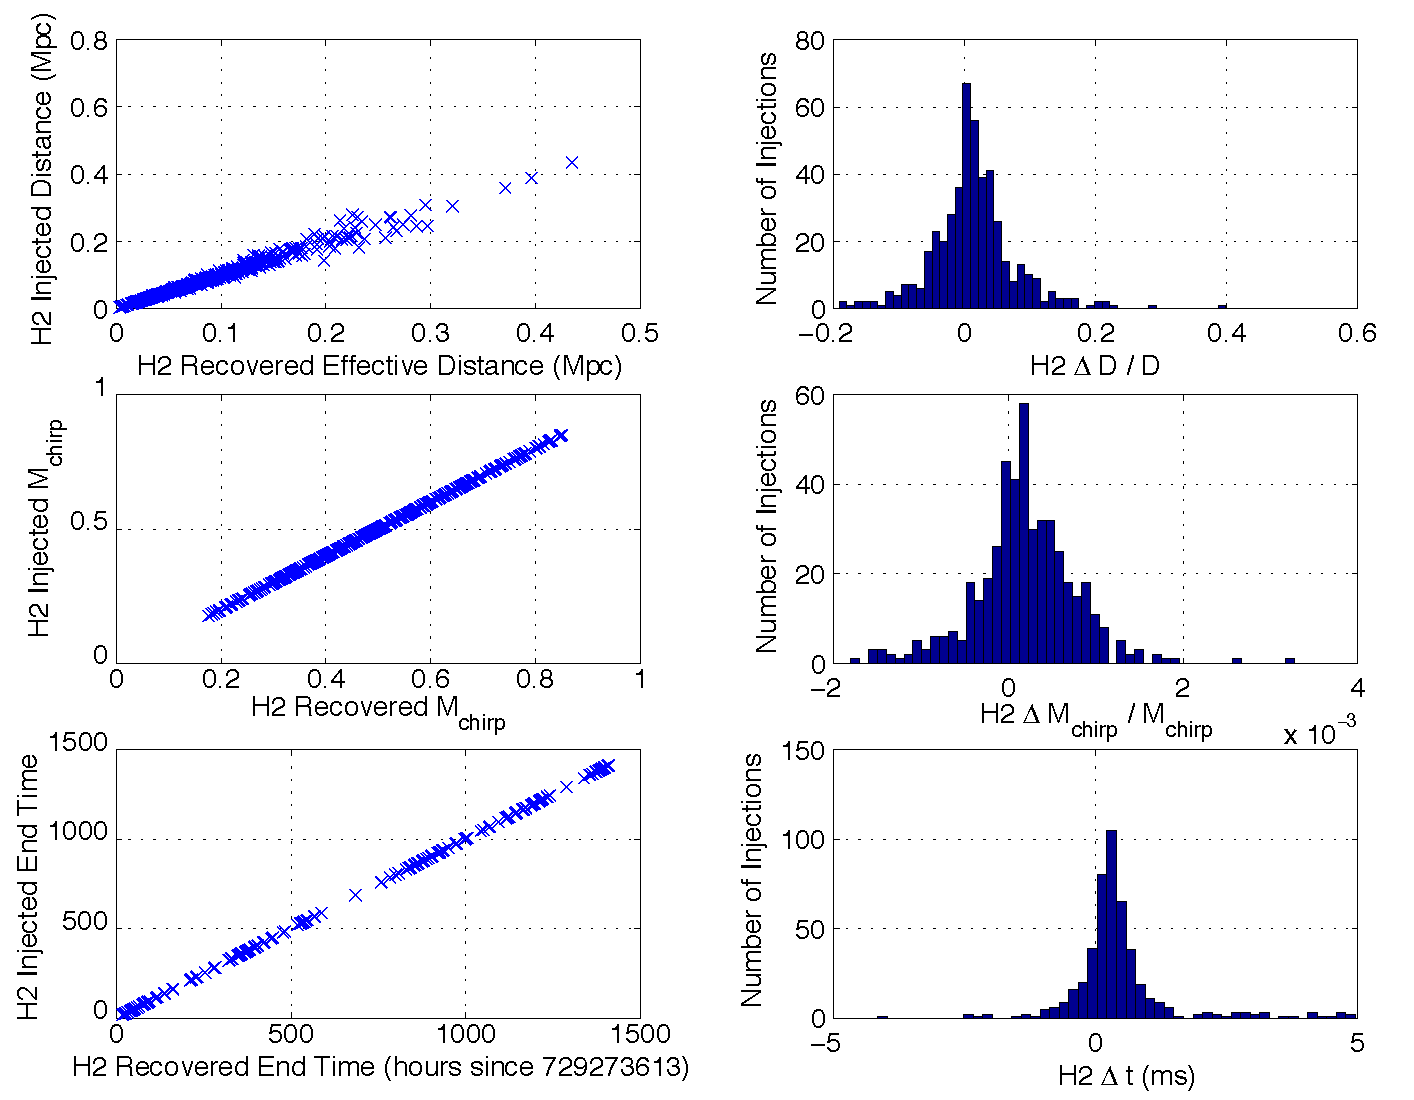
\includegraphics[width=\textwidth]{figures/result/h2_param_error}
\end{center}
\caption[Measurement accuracy of H2 Injections Parameters]{%
\label{f:h2_param_error}%
The panels in this figure compare the measured values of effective distance,
chirp mass and end time with the known values for the injected waveforms in
the Monte Carlo simulation in the H2 detector.
}
\end{figure}

\begin{figure}[p]
\begin{center}
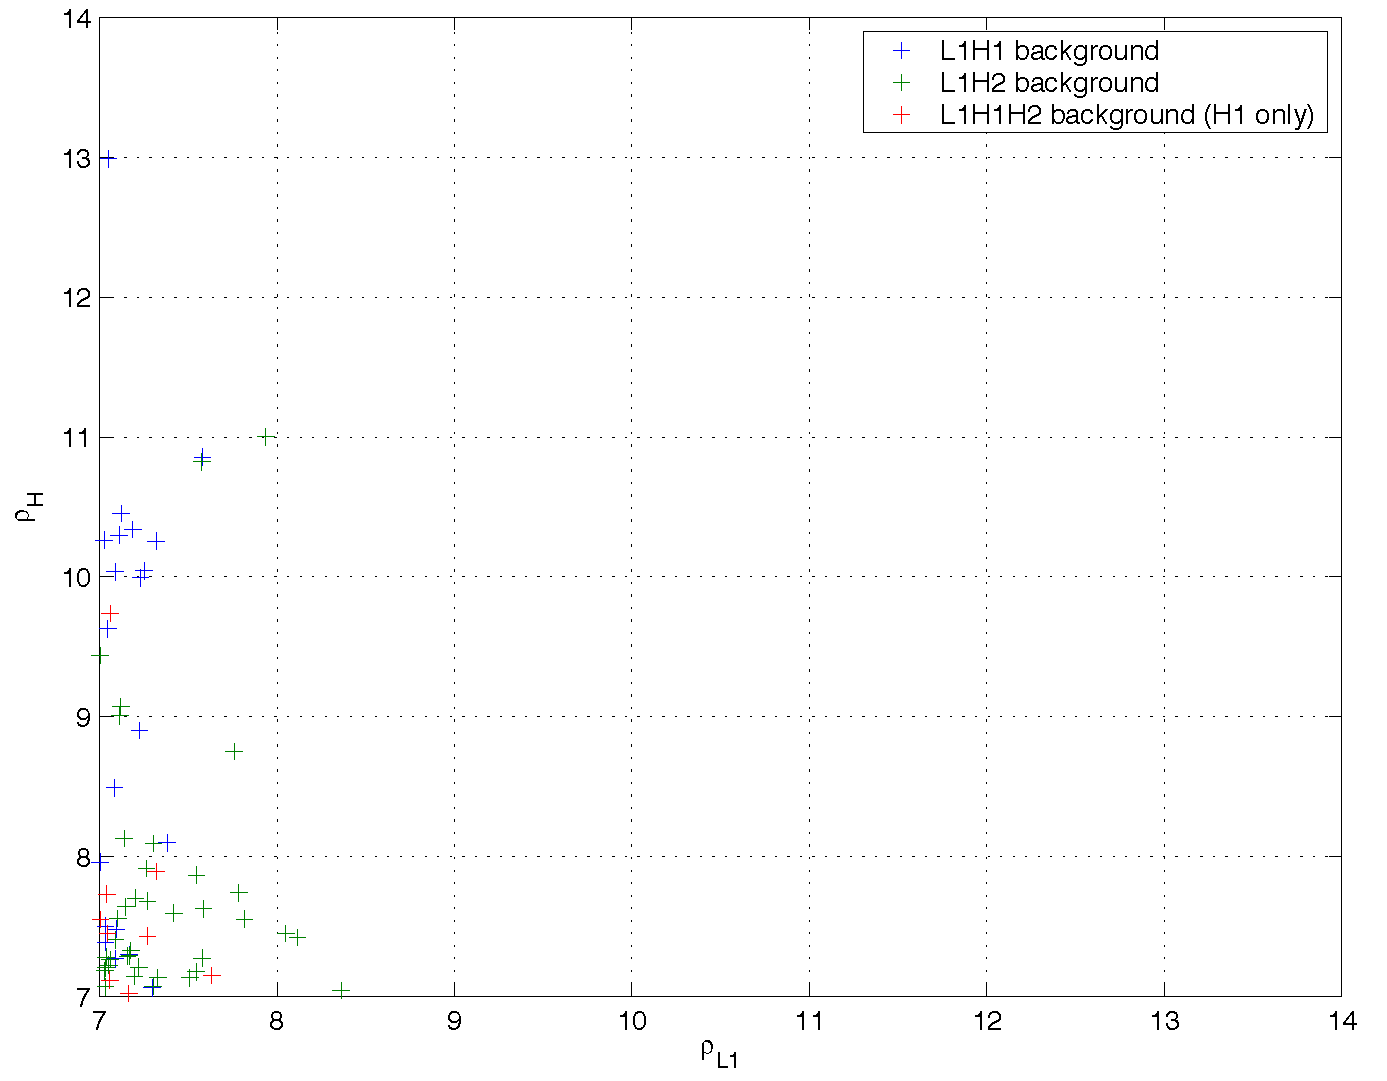
\includegraphics[width=\textwidth]{figures/result/bkg}
\end{center}
\caption[Background Triggers from 20 Time Slides]{%
\label{f:bkg}%
The signal-to-noise ratio of the background triggers produced by 20
time-slides. No triple coincident background triggers were observed.
The colors are color coded depending on whether they were found in the triple,
L1-H1 double of L1-H1 double triggers coincident data. No background triggers 
were found coincident in all three detectors, so the triggers from the triple
coincident data set are from L1-H1 coincidence only.
}
\end{figure}

\begin{figure}[p]
\begin{center}
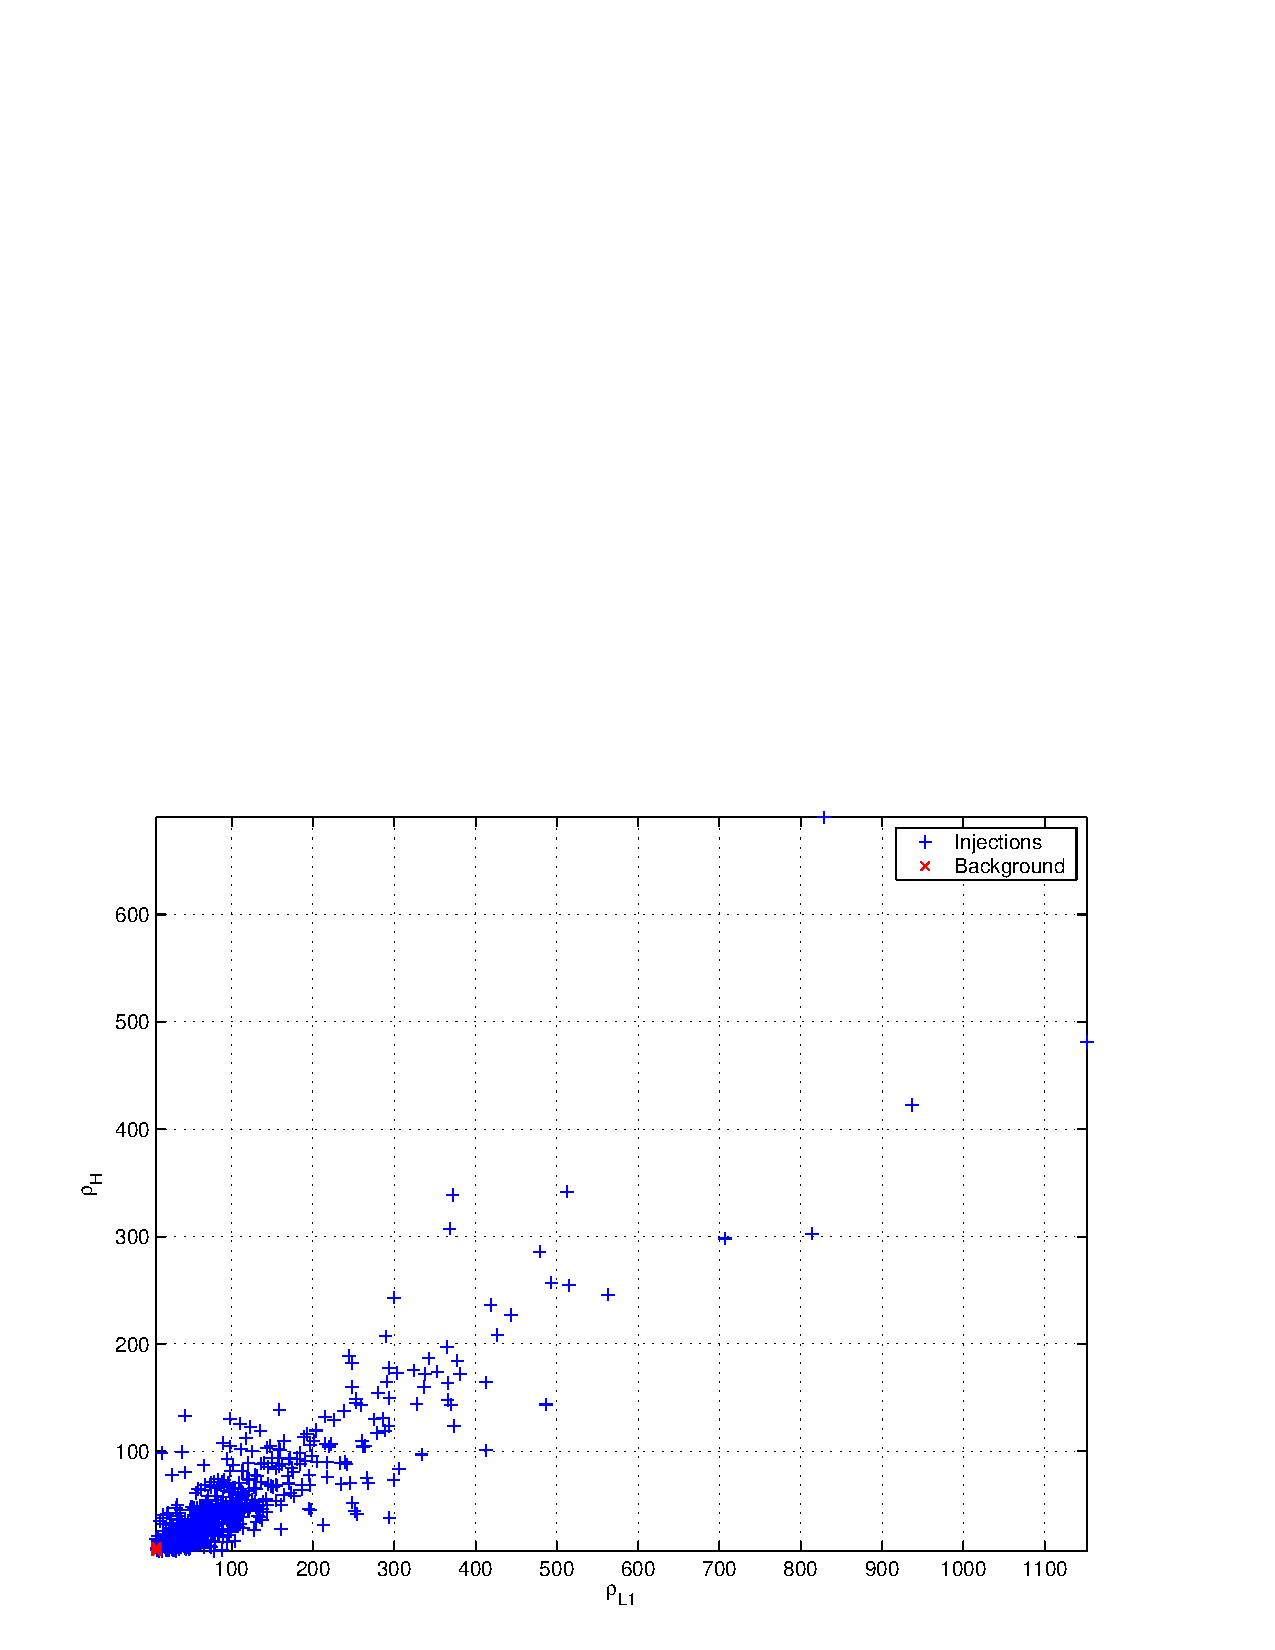
\includegraphics[width=0.7\textwidth]{figures/result/bkg_inj}\\
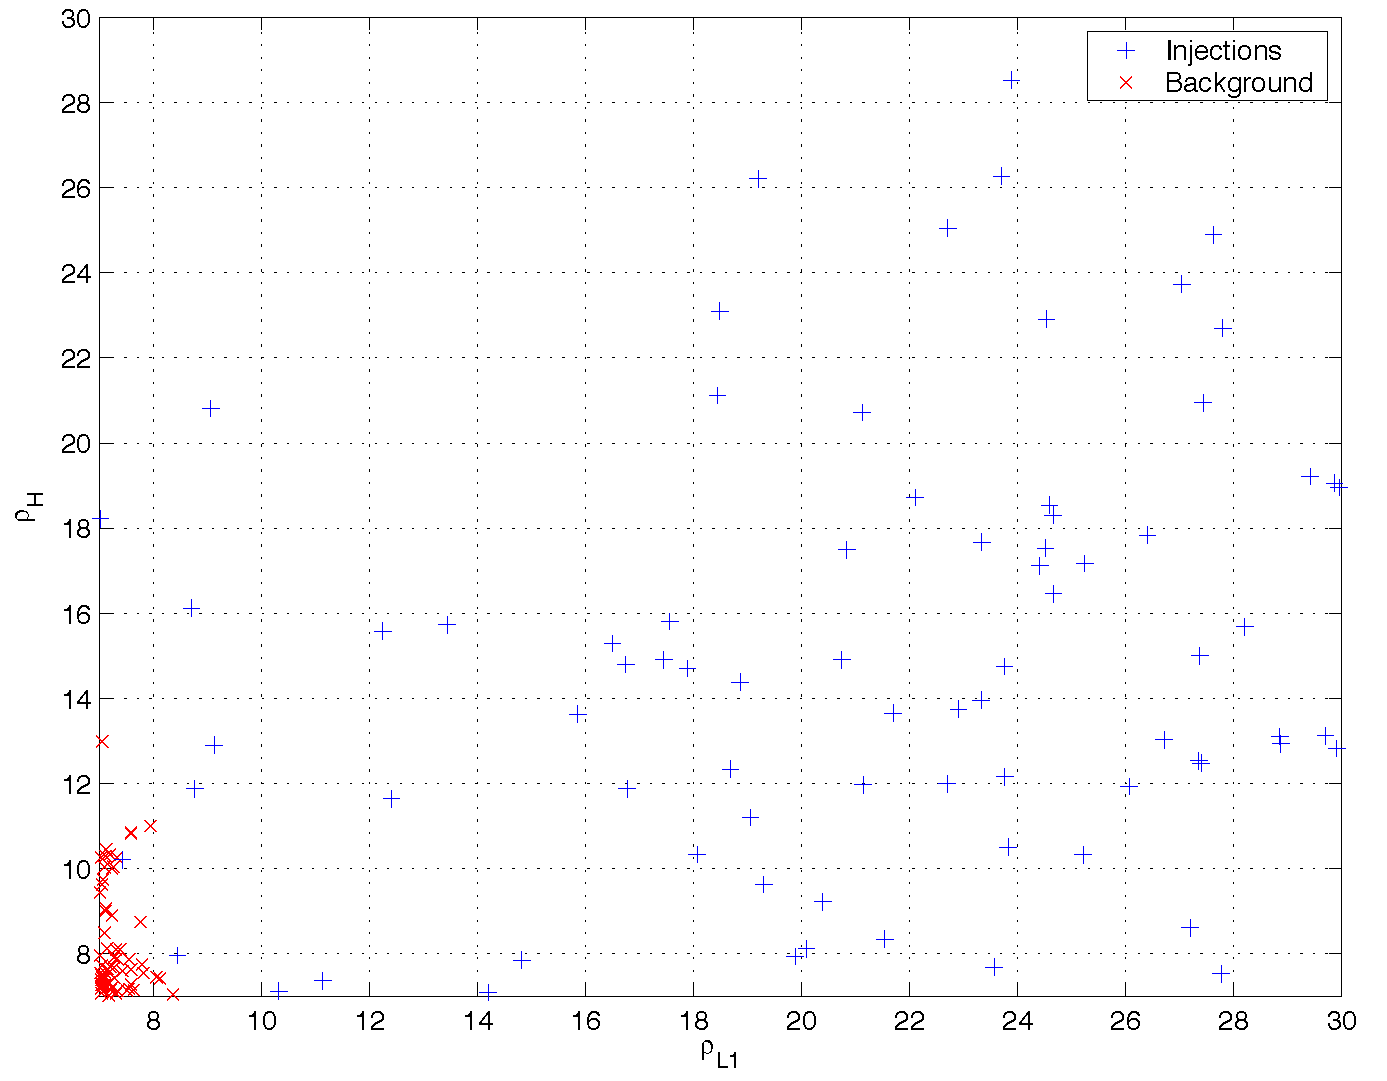
\includegraphics[width=0.7\textwidth]{figures/result/bkg_inj_zoom}
\end{center}
\caption[Comparison of Background Triggers and Injections]{%
\label{f:bkg_inj}%
The plots in this figure compare the signal-to-noise ratios of the background
triggers to those of the triggers corresponding to software injections from the
Monte Carlo simulation. Notice in the upper plot that the signal-to-noise
ratio of detected injections in L1 is a factor of $\sim 2$ higher than the
signal-to-noise ratio in the LHO detectors, due to the greater sensitivity of
L1. The lower plot shows a magnification of the low signal-to-noise ratio
region. It can be seen that background triggers generally have a larger
signal-to-noise ratio in the LHO detectors, suggesting the coherent statistic
described in the text that gives greater weight to the L1 signal-to-noise
ratio.
}
\end{figure}




